\chapter{传输机制评测}
\label{chap:evaluation}
\label{chap:simulation}
\label{sec:eval-simulation}

本章按机制组织传输层证据：每类 claim 先给出物理原型上的锚点（如有），
再由包级仿真扩展到物理设施无法承载的规模与故障矩阵。LLM 训练工作负载
的端到端评估单独构成 \cref{chap:llm-evaluation}。

\section{平台、方法与证据边界}
\label{ssec:eval-testbed}
\label{ssec:eval-setup}

\parab{物理平台.}
物理原型使用四台 DPDK endpoint、一台 Tofino 交换机和一块 Alveo
V80。Tofino 连接四个 100-GbE endpoint 端口和 V80 的四个 100-GbE
DCMAC 端口；单层主实验使用四个 rank、两个 replica、8-KiB 完整 FP32
payload 和 $A=1024$ 个物理聚合 row，两层实验在同一块 V80 上实现四个
逻辑交换机、host 端固定 40~Gbps。三个系统各自绑定冻结的 routed 镜像与
端点源码；镜像编号、逐实验绑定与完整审计流程见
\cref{app:physical-implementation-audit}。

物理结果的证据纪律统一如下。每个正式运行绑定镜像、二进制与配置哈希，
测量窗前后核对 Tofino、DCMAC 和 FPGA 计数器、逐跳帧守恒与四个 rank 的
确定性 FP32 结果；数值、身份或守恒失败使该次运行作废。重传、repair 和
owner miss 作为观测结果保留、不用重跑替换；可恢复且能精确归因的链路
缺口标为 recovery-qualified，而非物理零丢包。除特别说明外，每个物理
性能点运行五个新进程，报告中位数和完整极差；吞吐矩阵使用
cache-diverse 口径——warm-up 与正式迭代访问不同的预注册 buffer，避免
把 cache 驻留当作应用吞吐。requester 侧的 payload 交付路径（CPU 拷贝或
同 NUMA I/OAT DMA，\cref{sec:impl-structure}）按 primitive 和消息大小
在正式运行前冻结。本章凡小标题以「物理」开头的实验来自该平台并遵循
上述纪律，未标记的实验为包级仿真。

\parab{物理端侧 CPU 口径与 baseline 调优.}
\label{sssec:eval-endpoint-cpu}
物理实验以测量窗内持续执行协议数据面的 poller lcore 为 CPU 资源单位，
不计只负责发布与等待完成的 EAL main lcore。ATP 的 PS 与 worker 是
非对称角色，结果分别报告两类节点的 poller 数；图中标量横轴为全 job
poller 总数除以所有 endpoint 的线速总和（以 100~Gbps 为单位），不把该平均值
解释为每类节点使用相同核数。端侧扫描在相同的四 rank、100-GbE、64-MiB、
8-KiB payload 和 FP32 正确性门下进行（Arbor 在该实验关闭 CC 以隔离
endpoint service capacity；其余物理实验使用另行冻结的 Swift
profile），跨系统比较取五次重复均通过审计、中位吞吐达到 90~Gbps 的
最小已测配置。ATP 和 SwitchML 允许一切与协议语义无关的端侧优化——
NUMA-local 内存、多队列、批处理、消除冗余拷贝——但不引入 Arbor 的
credit、repair 或 allocator 机制；配置在读取结果前冻结，完整候选与
排除原因见 \cref{app:physical-implementation-audit}。

包级仿真在 ns-3.39 上实现完整的 multicast-credit 协议，包括逐级
slot/owner、\texttt{REGISTER}/\texttt{END}、normal/repair 双路径、
multi-subchannel 调度和 responder 侧拥塞控制。仿真器跟踪 payload
字节、贡献计数、owner 和提交状态，但不执行 FP32 数值运算——它检查的
是协议状态和单次提交，不验证 FP32 数值结果。

主要机制实验使用 128-host leaf-spine 或三层 fat-tree，规模实验使用
1024-host fat-tree。状态与单变量机制实验的 host 链路主要为 100~Gbps、
leaf-spine 为 200~Gbps；\cref{fig:baseline-anchor,fig:capstone-throughput}
另行固定全部链路为 200~Gbps。逐链路等效时延为 3~\textmu s，\sysname
的数据包携带 8-KiB payload。主实验开启 priority flow control（PFC），
并同时报告 peak queue 和累计 pause；PFC 仅提供无损保护，不替代端到端
控制。非 CC 机制实验使用 fixed-rate gate，其余分解实验使用 Swift。
每个 workload family 的候选都必须完成、无协议违例且无 packet drop；
PFC 作为观测结果报告，不是跨实验统一的排除条件。需要比较多 job 公平性的
实验另行预声明 Jain 门槛。选择只使用独立 calibration 点；冻结后，同一
配置用于该 family 的全部正式 seed 和机制对照。

除各实验另行定义外，一个 job 的 logical goodput 是其全部逻辑消息字节
除以该 job 从首次提交到最后完成的时间；aggregate logical goodput 使用
全部 job 的逻辑消息字节和全局 makespan。二者均按 collective 的逻辑
数据量计数，不把链路复制或协议 header 计入分子。

除各段另有说明外，主要随机敏感性实验运行 20 个配对 seed 并报告
Student-t 95\% CI；固定拓扑和事件序列的机制扫描运行一次。样本不足
$10^4$ 时报告 p90，不外推 p99。ATP-like、SwitchML-like 和 p2p-CCL 是
按论文关键报文与调度语义构建的包级模型，不代表相应系统的完整软硬件
实现；跨系统结果只作为量级锚点，\sysname 内部机制的收益由单变量消融
给出。概括地说：ATP-like 哈希寻址共享聚合表，冲突输入经 PS 补全，并
保留动态 remap、端侧 fallback 和恢复语义；SwitchML-like 为每个 job
构造固定的分层聚合树；p2p-CCL 是四条 NCCL-style ring 上的持久
RDMA/DCQCN 传输。前两者与 \sysname 同用 8-KiB payload 并移除量化与
反量化时延，使比较集中于寻址、状态分配和传输语义。三个模型的完整报文
语义、恢复行为与参数冻结流程见 \cref{app:sim-models}。

只有完成全部 collective，或满足预先声明的稳态 cohort 排空条件，并通过
协议断言的运行才进入正文；各段分别给出重复次数和统计口径。

\section{数据面吞吐、原语与多 job 并发}
\label{ssec:eval-throughput}
\label{ssec:eval-primitives}
\label{ssec:eval-capstone}

\parab{物理端侧核数：三系统跨过 90 Gbps 的最小配置.}
同为 90-Gbps 线速目标，\sysname 每 100-GbE endpoint 平均需要 2 个
poller（全 job 8 个），比 ATP-8K 的 5 个和 SwitchML-8K 的 8 个少
60\% 和 75\%，吞吐分别为 96.666、91.915 和 96.627~Gbps。ATP-8K 的
5 个是四个 endpoint 上的平均值：PS 使用 8 个，三个 worker 各使用 4 个，
全 job 共 20 个。完整曲线见 \cref{fig:physical-endpoint-pollers}，以最慢
rank 的 logical goodput 为任务速率：Arbor 和 SwitchML-8K 在每 100-GbE
endpoint 配置 1、2、4、8 个 poller；ATP-8K 的 PS/worker 配置
1/1、2/2、4/4、8/4、8/8 分别对应平均 1、2、4、5、8 个 poller。

\begin{figure}[t]
\centering
% Values are the five-process medians and full ranges from
% plots/data/pgf/poller-scan.csv.
\begin{tikzpicture}
\begin{axis}[
  arbor axis,
  width=\linewidth,height=0.60\linewidth,
  xmin=3,xmax=33,ymin=0,ymax=101,
  xtick={4,8,16,20,32},
  xlabel={全 job datapath poller 数},
  ylabel={AllReduce goodput (Gbps)},
  legend style={at={(0.98,0.04)},anchor=south east},
]
\addplot[ArborGray,dotted,forget plot] coordinates {(4,90) (32,90)};
\addplot[ArborBlue,thick,mark=*,mark options={fill=ArborBlue},
  error bars/.cd,y dir=both,y explicit]
table[row sep=\\,x=pollers,y=median,
  y error minus=minus,y error plus=plus] {
pollers median minus plus\\
4 46.588 0.056 0.023\\
8 96.666 0.271 0.319\\
16 97.501 0.026 0.023\\
32 97.471 0.046 0.035\\
};
\addlegendentry{Arbor}
\addplot[ArborOrange,thick,dashed,mark=square*,
  mark options={fill=ArborOrange},error bars/.cd,y dir=both,y explicit]
table[row sep=\\,x=pollers,y=median,
  y error minus=minus,y error plus=plus] {
pollers median minus plus\\
4 36.391 0.025 0.020\\
8 57.767 9.889 0.545\\
16 87.758 3.735 0.822\\
20 91.915 1.458 0.517\\
32 94.961 1.259 0.389\\
};
\addlegendentry{ATP-8K}
\addplot[ArborGreen,thick,dash dot,mark=triangle*,
  mark options={fill=ArborGreen},error bars/.cd,y dir=both,y explicit]
table[row sep=\\,x=pollers,y=median,
  y error minus=minus,y error plus=plus] {
pollers median minus plus\\
4 29.987 0.021 0.035\\
8 47.805 0.121 0.254\\
16 56.731 4.356 1.023\\
32 96.627 0.240 0.067\\
};
\addlegendentry{SwitchML-8K}
\end{axis}
\end{tikzpicture}

\caption{三个物理系统对端侧 poller 数的敏感度。workload 为 $N=4$、
$J=1$、$A=1024$、64-MiB FP32 AllReduce；点为五个新进程的中位数，
误差线为完整极差，虚线为 90-Gbps 目标。横轴是全 job datapath poller
总数除以所有 endpoint 的线速总和（以 100~Gbps 为单位）；该归一化消除
增加 endpoint 数量带来的平凡线性增长。ATP 的横轴 5 对应 PS 8 个、
三个 worker 各 4 个，
并非每台主机均使用 5 个。SwitchML 的整批窗口包含 $17.86$~ppm 可恢复
上行丢包。}
\label{fig:physical-endpoint-pollers}
\end{figure}

Arbor p1 的五次运行均数值正确，但中位吞吐只有 46.588~Gbps，并触发
responder stall recovery；该点保留在完整曲线中。

SwitchML-8K 的核数差异不来自交换机侧聚合，而来自端侧 per-slot 周转
位于其自时钟进度路径上：poller 收到聚合结果后必须校验并迁移 slot
状态、把 8-KiB 结果落入连续输出缓冲区，再生成并序列化该 slot 的下一份
贡献——该 slot 的后续输入要等这条链走完才被释放。在消除了可判定的
冗余开销之后，保留快路径仍需约 5.2--5.7k cycles/packet（不含 RX
burst、decode 与 timer；完整端侧关键路径审计见
\cref{app:physical-implementation-audit}），p8 靠并行更多独立 slot
周转达到线速。\sysname 的 credit 则把多个 offset 的发放、requester
贡献发送和 result completion 解耦，已注册的 contribution slice 可直接
作为 extbuf 发送，不必在同一个 response callback 中先落位结果、再复制
下一份 TX payload。这里报告的是优化后 CPU/DPDK 实现在本机 mlx5 数据
路径上的实测需求，不是 SwitchML 算法的固有核数下界。

在同一最小 R2/P2 配置下，五种原语与六种消息大小的完整笛卡尔积均使用
五个新进程验证；每种原语沿用正式运行前冻结的参数。该矩阵检验最小
poller 配置是否覆盖完整 API，而不参与 poller 数的选择。完整结果、
Reduce 的 P2/P4 对照和链路等效吞吐换算见
\cref{app:physical-implementation-audit,tab:physical-workload}。

\begin{table*}[t]
\centering
\small
\caption{三个物理系统的 AllReduce 消息大小矩阵。括号内为全系统
datapath poller 数：Arbor 每 rank 2 个（共 8 个），ATP 的 PS 为 8 个、
三个 worker 各 4 个（共 20 个），SwitchML 每 rank 8 个（共 32 个）。
三者均为 $N=4$、$J=1$、$A=1024$；每格报告五个新进程的中位 logical
goodput（Gbps）。该表等量约束物理聚合状态而非端侧 CPU。}
\label{tab:physical-allreduce-size}
\setlength{\tabcolsep}{7pt}
\resizebox{\linewidth}{!}{%
\begin{tabular}{lrrr}
\toprule
消息大小 & \sysname（8 poller） & ATP-8K（20 poller） &
SwitchML-8K（32 poller） \\
\midrule
64 KiB & 7.489 & 7.273 & 7.853 \\
256 KiB & 23.622 & 21.179 & 24.655 \\
1 MiB & 50.890 & 44.083 & 52.394 \\
4 MiB & 77.749 & 74.460 & 72.131 \\
16 MiB & 90.359 & 89.044 & 91.774 \\
64 MiB & 97.217 & 91.608 & 96.429 \\
\bottomrule
\end{tabular}}
\end{table*}

\parab{物理单层多 job 与成员规模.}
两个完全重合的四-rank job 使用同一 Swift 参数和每 job 四个 poller：
并发时存活 job 的两个方向中位吞吐均为 44.734~Gbps，对端 job 离开后
分别恢复到 97.151 和 97.069~Gbps，新批次开始复用释放容量的最长观测
时间为 5.318~ms；十次预定重复的 80 个结果全部数值精确并通过硬件守恒
门。三-rank 实验改用 $\{H_0,H_1,H_2\}$ 和 $\{H_1,H_2,H_3\}$ 两个部分
重合的 job 而不改 CC 参数：每 job 从四个 poller 增至六个后，较慢的
solo 中位吞吐从 89.407 升至 96.297~Gbps，而双 job aggregate 仅从
97.804 变为 97.933~Gbps——低 solo 点因此来自两条 channel 共用一个
poller 的 endpoint serialization，不是 CC 失配。六-poller handoff
中，存活 job 从 44.727--44.729 恢复到 97.392--97.409~Gbps。这些结果
支持一个 64-MiB batch（约 5.5~ms）粒度内的容量复用，分辨不了更细的
时间行为；更细粒度由两层实验与仿真承担。

\parab{原语、组规模与消息大小.}
包级仿真的单 job 扫描运行 AllReduce、Reduce、ReduceScatter、
Broadcast 和 AllGather，覆盖 $N=4$--128 和 64~KiB--1~GiB；Barrier
单独运行 100 次。187 个配置均无协议违例。64-MiB AllReduce 在
$N=16,64,128$ 时分别达到 96.6、92.9 和 87.2~Gbps，1-GiB 消息分别达到
99.1、98.9 和 98.3~Gbps；64-KiB 消息只有 7.4--7.8~Gbps，小消息区由
闭环启动和有限包数主导。64-MiB 和 1-GiB 代表点分别不低于 87.2 和
98.3~Gbps；本文逐组规模报告，不假设吞吐随 $N$ 单调变化。

\parab{拓扑深度与公平设置.}
跨系统仿真固定 128 个 200-Gbps endpoint、3~\textmu s 单向链路时延和
256-MiB AllReduce。一个 job 含 16 个 ranks；一层控制把 ranks 接入同一
聚合交换机，两层拓扑含 4 台 access 和 4 台 root，三层拓扑含 8 台 ToR、
4 台 leaf 和 4 台 root。两层中每个 job 在每台 access 下放 4 个 ranks；
三层中每台 ToR 放 2 个。两/三层的上层均提供 4 条 200-Gbps 候选路径，
八 job 的 post-aggregation offered load 与该 800-Gbps cut 之比为 2:1；
三层的 ToR--leaf bundle 不构成额外瓶颈。

三个 INC 模型在每台可聚合交换机使用相同的 12-MiB 物理状态和 8-KiB
payload。ATP-like 由通信组内一个 rank 兼任 PS，不增加 endpoint 或 NIC，
并只在 worker/PS ToR 聚合；SwitchML-like 为每个 job 使用一棵固定分层
树；\sysname 在两/三层为每个 job 预先配置全部四棵候选树，再按运行时
反馈分配 packet offset。SwitchML-like 使用全局均衡的最优静态 root
映射，NCCL-like 使用四条 topology-aware ring。

\parab{单 job 深度控制.}
\Cref{fig:baseline-anchor} 比较一个持续通信的 16-rank job；纵轴直接报告
logical goodput，不对层数作协议相关换算。一层中，ATP-like、
SwitchML-like 和 \sysname 分别达到 198.31、198.43 和 196.25~Gbps，
NCCL-like 为 103.73~Gbps。两层中四者分别为 97.94、198.31、197.17 和
102.83~Gbps；三层为 94.14、198.19、195.83 和 101.95~Gbps。固定分层树在
该静态场景中最快；\sysname 在三种深度均达到 endpoint rate 的
97.9\%--98.6\%，与 SwitchML-like 相差 0.6\%--1.2\%。

\begin{figure}[t]
\centering
\begin{tikzpicture}
\begin{axis}[
  arbor axis,
  width=0.84\linewidth,height=0.50\linewidth,
  xmin=-0.15,xmax=2.15,ymin=0,ymax=210,
  xtick={0,1,2},xticklabels={One tier,Two tiers,Three tiers},
  ylabel={Logical goodput (Gbps)},
  legend style={at={(0.5,1.03)},anchor=south,legend columns=4,
    /tikz/every even column/.append style={column sep=5pt}},
]
\addplot[black,densely dotted,no marks,forget plot]
  coordinates {(0,200) (2,200)};
\addplot[ArborGray,thick,dotted,mark=triangle*,
  error bars/.cd,y dir=both,y explicit]
  table[col sep=comma,x=x,y=nccl,y error=nccl_error]
    {plots/data/pgf/transport-depth-single.csv};
\addlegendentry{NCCL-like}
\addplot[ArborOrange,thick,dashed,mark=square*,
  error bars/.cd,y dir=both,y explicit]
  table[col sep=comma,x=x,y=atp,y error=atp_error]
    {plots/data/pgf/transport-depth-single.csv};
\addlegendentry{ATP-like}
\addplot[ArborGreen,thick,dash dot,mark=diamond*,
  error bars/.cd,y dir=both,y explicit]
  table[col sep=comma,x=x,y=switchml,y error=switchml_error]
    {plots/data/pgf/transport-depth-single.csv};
\addlegendentry{SwitchML-like}
\addplot[ArborBlue,thick,mark=*,
  error bars/.cd,y dir=both,y explicit]
  table[col sep=comma,x=x,y=arbor,y error=arbor_error]
    {plots/data/pgf/transport-depth-single.csv};
\addlegendentry{Arbor}
\end{axis}
\end{tikzpicture}

\caption{一、二、三层拓扑上的单-job AllReduce。每点为五次配对运行的
均值，误差线为 Student-t 95\% CI；黑色虚线为 200-Gbps endpoint rate。
每次运行包含四轮 256-MiB AllReduce。}
\label{fig:baseline-anchor}
\end{figure}

ATP-like 只在 ToR 聚合，partial results 仍需经上层网络到达组内 PS；
SwitchML-like 和 \sysname 则在各层执行聚合。因此，增加拓扑深度只使
ATP-like 的单-job goodput 下降约一半。

\parab{暂时空闲通信组的路径复用.}
八个互不共享 NIC 的 job 使用同一拓扑和 256-MiB 消息。51.2-ms warm-up
之后，14 个 51.2-ms epoch 每次允许四个 job 启动下一轮 collective；每个 job
出现 7 次，任意 job 对共同出现 3 次。活动集合只在 collective 边界改变：
已经启动的 AllReduce 排空，关闭的 job 不再启动后继。该 50\%-active
输入取自训练通信组约 60\%--85\% 空闲时间的保守抽象；统计量为
51.2--768~ms 固定窗口内完成的 logical bytes 除以窗口长度，不除以
50\%。

\begin{figure}[t]
\centering
\begin{tikzpicture}
\begin{axis}[
  arbor axis,
  width=0.84\linewidth,height=0.50\linewidth,
  xmin=-0.15,xmax=2.15,ymin=0,ymax=900,
  xtick={0,1,2},xticklabels={One tier,Two tiers,Three tiers},
  ylabel={Aggregate logical goodput (Gbps)},
  legend style={at={(0.5,1.03)},anchor=south,legend columns=4,
    /tikz/every even column/.append style={column sep=5pt}},
]
\addplot[ArborGray,thick,dotted,mark=triangle*,
  error bars/.cd,y dir=both,y explicit]
  table[col sep=comma,x=x,y=nccl,y error=nccl_error]
    {plots/data/pgf/transport-depth-multijob.csv};
\addlegendentry{NCCL-like}
\addplot[ArborOrange,thick,dashed,mark=square*,
  error bars/.cd,y dir=both,y explicit]
  table[col sep=comma,x=x,y=atp,y error=atp_error]
    {plots/data/pgf/transport-depth-multijob.csv};
\addlegendentry{ATP-like}
\addplot[ArborGreen,thick,dash dot,mark=diamond*,
  error bars/.cd,y dir=both,y explicit]
  table[col sep=comma,x=x,y=switchml,y error=switchml_error]
    {plots/data/pgf/transport-depth-multijob.csv};
\addlegendentry{SwitchML-like}
\addplot[ArborBlue,thick,mark=*,
  error bars/.cd,y dir=both,y explicit]
  table[col sep=comma,x=x,y=arbor,y error=arbor_error]
    {plots/data/pgf/transport-depth-multijob.csv};
\addlegendentry{Arbor}
\end{axis}
\end{tikzpicture}

\caption{八个 job 在 50\%-active 通信组轨迹下的 fixed-window aggregate
logical goodput。每点为五次配对运行的均值，误差线为 Student-t 95\%
CI。SwitchML-like 使用离线最优的均衡固定树映射；\sysname 的四棵候选树
同样在运行前固定。}
\label{fig:capstone-throughput}
\end{figure}

一层没有路径选择，\sysname 与 SwitchML-like 均为 850.85~Gbps。该值可
高于四个 launch-eligible job 的 800~Gbps 名义速率：活动边界前已启动的
collective 会与新一组 job 短暂重叠，因此 800~Gbps 不是一层的物理上界。
两层中，\sysname 达到 763.96~Gbps，SwitchML-like 为 653.11~Gbps；三层
分别为 754.97 和 653.11~Gbps，提升为 17.0\% 和 15.6\%。这对应共享
800-Gbps upper cut 的 95.5\% 和 94.4\%。一层相同而多层
分离，说明收益来自反馈把后续 offset 移到当前空闲的预配置 root，而非不同
的 endpoint、消息或状态容量。

NCCL-like 在一/二/三层分别达到 467.37、230.69 和 232.48~Gbps；
ATP-like 为 505.11、146.20 和 80.29~Gbps。

后续小节分别隔离共享状态、反馈驱动选树、拥塞控制和恢复机制。

\section{多租户共享与聚合状态定容}
\label{ssec:eval-state}
\label{ssec:eval-multitenant}

\parab{物理状态与并发 job.}
我们在三个系统各自的冻结镜像上扫描 8-KiB 物理聚合 row 数
$A=8,16,\ldots,160$，并分别运行 $J\in\{1,2,4\}$ 个独立的四-rank、
64-MiB AllReduce job。Arbor 和 ATP 的横轴分别为 active row 和 hash
row；SwitchML 的每个逻辑 slot 使用两个 generation bank，按 $A=2K$ 个
物理 row 计数。每个 $(\text{system},A,J)$ 点以冻结参数运行五次正式
重复，180 个 cell、共 900 个正式进程全部通过数值与硬件门，恢复事件
保留在样本中。各系统保持原生端侧配置，该实验因此比较相同物理状态预算
下的吞吐，不作等 CPU 声明。

\begin{figure*}[t]
\centering
\pgfplotstableread[col sep=comma]
  {plots/data/pgf/physical-state-jobs.csv}\physicalstatejobsdata
\IfFileExists{plots/data/pgf/physical-state-jobs-ready.tex}
  {% The sealed three-system join has populated all baseline columns.
\def\physicalstatehasbaselines{1}
}
  {\def\physicalstatehasbaselines{0}}

\begin{tikzpicture}
\begin{groupplot}[
  group style={group size=3 by 1,horizontal sep=0.025\textwidth},
  arbor axis,
  arbor panel,
  width=0.315\textwidth,height=0.30\textwidth,
  xmin=4,xmax=164,ymin=0,ymax=102,
  xtick={8,32,64,96,128,160},
  xticklabel style={font=\scriptsize},
  ytick={0,20,40,60,80,100},
  xlabel={Physical 8-KiB rows $A$},
]
\nextgroupplot[
  title={(a) $J=1$},
  ylabel={Aggregate goodput (Gbps)},
  legend to name=physicalstatejobslegend,
  legend columns=3,
  legend style={/tikz/every even column/.append style={column sep=5pt}},
]
\addplot[ArborGray,dotted,forget plot] coordinates {(8,100) (160,100)};
\addplot[ArborBlue,thick,mark=*,mark size=1.5pt,
  error bars/.cd,y dir=both,y explicit]
  table[col sep=comma,x=physicalA,y=arborMedian,
    y error minus=arborMinus,y error plus=arborPlus,
    restrict expr to domain={\thisrow{jobs}}{1:1}]
    {\physicalstatejobsdata};
\addlegendentry{Arbor}
\ifnum\physicalstatehasbaselines=1
\addplot[ArborOrange,thick,dashed,mark=square*,mark size=1.4pt,
  unbounded coords=jump,error bars/.cd,y dir=both,y explicit]
  table[x=physicalA,y=atpMedian,
    y error minus=atpMinus,y error plus=atpPlus,
    restrict expr to domain={\thisrow{jobs}}{1:1}]
    {\physicalstatejobsdata};
\addlegendentry{ATP-8K}
\addplot[ArborGreen,thick,dash dot,mark=triangle*,mark size=1.5pt,
  unbounded coords=jump,error bars/.cd,y dir=both,y explicit]
  table[x=physicalA,y=switchmlMedian,
    y error minus=switchmlMinus,y error plus=switchmlPlus,
    restrict expr to domain={\thisrow{jobs}}{1:1}]
    {\physicalstatejobsdata};
\addlegendentry{SwitchML-8K}
\fi

\nextgroupplot[
  title={(b) $J=2$},
  yticklabels={},
]
\addplot[ArborGray,dotted,forget plot] coordinates {(8,100) (160,100)};
\addplot[ArborBlue,thick,mark=*,mark size=1.5pt,
  error bars/.cd,y dir=both,y explicit]
  table[col sep=comma,x=physicalA,y=arborMedian,
    y error minus=arborMinus,y error plus=arborPlus,
    restrict expr to domain={\thisrow{jobs}}{2:2}]
    {\physicalstatejobsdata};
\ifnum\physicalstatehasbaselines=1
\addplot[ArborOrange,thick,dashed,mark=square*,mark size=1.4pt,
  unbounded coords=jump,error bars/.cd,y dir=both,y explicit]
  table[x=physicalA,y=atpMedian,
    y error minus=atpMinus,y error plus=atpPlus,
    restrict expr to domain={\thisrow{jobs}}{2:2}]
    {\physicalstatejobsdata};
\addplot[ArborGreen,thick,dash dot,mark=triangle*,mark size=1.5pt,
  unbounded coords=jump,error bars/.cd,y dir=both,y explicit]
  table[x=physicalA,y=switchmlMedian,
    y error minus=switchmlMinus,y error plus=switchmlPlus,
    restrict expr to domain={\thisrow{jobs}}{2:2}]
    {\physicalstatejobsdata};
\fi

\nextgroupplot[
  title={(c) $J=4$},
  yticklabels={},
]
\addplot[ArborGray,dotted,forget plot] coordinates {(8,100) (160,100)};
\addplot[ArborBlue,thick,mark=*,mark size=1.5pt,
  error bars/.cd,y dir=both,y explicit]
  table[col sep=comma,x=physicalA,y=arborMedian,
    y error minus=arborMinus,y error plus=arborPlus,
    restrict expr to domain={\thisrow{jobs}}{4:4}]
    {\physicalstatejobsdata};
\ifnum\physicalstatehasbaselines=1
\addplot[ArborOrange,thick,dashed,mark=square*,mark size=1.4pt,
  unbounded coords=jump,error bars/.cd,y dir=both,y explicit]
  table[x=physicalA,y=atpMedian,
    y error minus=atpMinus,y error plus=atpPlus,
    restrict expr to domain={\thisrow{jobs}}{4:4}]
    {\physicalstatejobsdata};
\addplot[ArborGreen,thick,dash dot,mark=triangle*,mark size=1.5pt,
  unbounded coords=jump,error bars/.cd,y dir=both,y explicit]
  table[x=physicalA,y=switchmlMedian,
    y error minus=switchmlMinus,y error plus=switchmlPlus,
    restrict expr to domain={\thisrow{jobs}}{4:4}]
    {\physicalstatejobsdata};
\fi

% The sealed installer adds the baseline columns only after both fresh scans
% pass. SwitchML's x value is already charged both physical version banks.
\end{groupplot}
\node[anchor=south,yshift=26pt] at (group c2r1.north)
  {\ref{physicalstatejobslegend}};
\end{tikzpicture}

\caption{物理聚合状态随并发 job 数的吞吐变化。三个面板分别固定
$J=1,2,4$；横轴按实际的 8-KiB 物理 row 计数，纵轴为所有并发 job 的
aggregate logical goodput。点为五次正式重复的中位数，误差线为完整极差；
虚线为 100-Gbps 链路速率。端侧 poller 不作等量约束：Arbor 每 job、
每 rank 使用 4 个（$J=1,2,4$ 时全系统为 16、32、64 个）；ATP 使用
8 个 PS poller 和三个 worker 各 4 个（共 20 个）；SwitchML 在 $A=8$
时每 rank 4 个（共 16 个），其余点每 rank 8 个（共 32 个）。因此该图
比较同物理状态预算下的吞吐，不作等 CPU 性能声明。}
\label{fig:physical-state-jobs}
\end{figure*}

\Cref{fig:physical-state-jobs} 显示，Arbor 超过一个随 $J$ 缓慢右移的状态
拐点后稳定在 95--98~Gbps。以每个 $J$ 的 $A=160$ 中位吞吐作为状态充足
参考，并要求该点及所有更大的已测 $A$ 均保持至少 95\%，Arbor 在
$J=1,2,4$ 时分别只需 48、56 和 64 个物理 row。$J=1$ 时，ATP 和
SwitchML 达到各自最佳中位吞吐 95\% 的持久定容点均为 $A=112$，Arbor
为 $A=48$。在公共预算 $A=128$ 下，Arbor、ATP 和 SwitchML 的 $J=1$
中位吞吐分别为 97.176、91.982 和 95.478~Gbps；$J=2$ 时为
96.844、51.104 和 95.878~Gbps，$J=4$ 时为 96.861、49.979 和
96.175~Gbps。该判据允许协议恢复，刻画的是吞吐定容点，不是零恢复点。

Arbor 的十五次 $A=128$ 运行均落在 96.580--97.319~Gbps。
3,440,640 次 allocation 中有 323 次 owner miss（93.878~ppm），140/140 个
rank-job 结果均精确；该点是 recovery-qualified 线速点，不作
owner-miss-free 声明。ATP 在相同预算下增加 $J$ 后仍停留在约
50~Gbps，而 SwitchML 和 Arbor 保持 95~Gbps 以上。由于三者使用的端侧
poller 数并不相同，该结果是原生配置下的系统级状态敏感度，不能单独量化
allocator 相对等 CPU baseline 的收益。

并发数本身不是吞吐下降的充分原因：在很小的 $A$ 下，更多独立 job 反而
提高 aggregate goodput。真正的变量是各 job 独立 credit window 叠加成的
短时分配序列——其工作集超过循环 allocator 的复用距离时，owner miss
与恢复工作才增加。对十个异常点单独追加的诊断扫描（不混入主曲线）给出
直接证据：$A=48$ 时，$J=1,2,4$ 的吞吐最优初始 credit 窗口 $W_0$ 分别
为 4、2、1，即三种并发共享同一份 $8JW_0=32$ 的名义启动授权量（每 job
八条物理 channel），正式中位吞吐为 95.564、91.247 和 91.141~Gbps。该
授权量不等同于同时占用量，正确性仍由 \cref{sssec:slot-bound} 的
allocation-sequence reuse 条件决定；这些点支持``并发 credit 窗口改变
状态拐点''的解释，但不能单独归因为 RTT 增长。

\parab{物理在线复用已释放状态.}
我们使用独立于本实验选出的公共预算 $A=128$，同时运行一个 64-MiB donor
和一个 256-MiB survivor。Donor 完成后，survivor 在同一进程内继续提交
offset；端点、CC 状态和控制面配置均不重启。Arbor 的两个 job 共享一个
owner-tagged pool；ATP-8K 的两个 job 以独立 window hash 到同一张物理表；
SwitchML-8K 则保留运行开始时确定的静态连续分区。每个系统反转 donor 方向，
每个方向运行五次。

\begin{figure}[t]
\centering
\pgfplotstableread[col sep=comma]
  {plots/data/pgf/physical-state-handoff-timeseries.csv}\physicalstatehandoffdata

\begin{tikzpicture}
\begin{axis}[
  arbor axis,
  axis on top,
  width=\linewidth,height=0.61\linewidth,
  xmin=-8,xmax=10,ymin=0,ymax=103,
  xtick={-8,-4,0,4,8},
  ytick={0,20,40,60,80,100},
  xlabel={Time from donor completion (ms)},
  ylabel={Survivor goodput (Gbps)},
  legend style={at={(0.5,1.03)},anchor=south,legend columns=3,
    /tikz/every even column/.append style={column sep=4pt}},
]
\addplot[ArborGray,dotted,forget plot] coordinates {(-8,100) (10,100)};

\addplot[name path=arborHandoffUpper,draw=none,forget plot]
  table[x=time_ms,y=q3_gbps,
    restrict expr to domain={\thisrow{system_id}}{0:0}]
    {\physicalstatehandoffdata};
\addplot[name path=arborHandoffLower,draw=none,forget plot]
  table[x=time_ms,y=q1_gbps,
    restrict expr to domain={\thisrow{system_id}}{0:0}]
    {\physicalstatehandoffdata};
\addplot[fill=ArborBlue,fill opacity=0.13,draw=none,forget plot]
  fill between[of=arborHandoffUpper and arborHandoffLower];

\addplot[name path=atpHandoffUpper,draw=none,forget plot]
  table[x=time_ms,y=q3_gbps,
    restrict expr to domain={\thisrow{system_id}}{1:1}]
    {\physicalstatehandoffdata};
\addplot[name path=atpHandoffLower,draw=none,forget plot]
  table[x=time_ms,y=q1_gbps,
    restrict expr to domain={\thisrow{system_id}}{1:1}]
    {\physicalstatehandoffdata};
\addplot[fill=ArborOrange,fill opacity=0.10,draw=none,forget plot]
  fill between[of=atpHandoffUpper and atpHandoffLower];

\addplot[name path=switchmlHandoffUpper,draw=none,forget plot]
  table[x=time_ms,y=q3_gbps,
    restrict expr to domain={\thisrow{system_id}}{2:2}]
    {\physicalstatehandoffdata};
\addplot[name path=switchmlHandoffLower,draw=none,forget plot]
  table[x=time_ms,y=q1_gbps,
    restrict expr to domain={\thisrow{system_id}}{2:2}]
    {\physicalstatehandoffdata};
\addplot[fill=ArborGreen,fill opacity=0.10,draw=none,forget plot]
  fill between[of=switchmlHandoffUpper and switchmlHandoffLower];

\addplot[ArborBlue,very thick]
  table[x=time_ms,y=median_gbps,
    restrict expr to domain={\thisrow{system_id}}{0:0}]
    {\physicalstatehandoffdata};
\addlegendentry{Arbor}
\addplot[ArborOrange,very thick,dashed]
  table[x=time_ms,y=median_gbps,
    restrict expr to domain={\thisrow{system_id}}{1:1}]
    {\physicalstatehandoffdata};
\addlegendentry{ATP-8K}
\addplot[ArborGreen,very thick,dash dot]
  table[x=time_ms,y=median_gbps,
    restrict expr to domain={\thisrow{system_id}}{2:2}]
    {\physicalstatehandoffdata};
\addlegendentry{SwitchML-8K}

\draw[ArborGray,densely dashed] (axis cs:0,0) -- (axis cs:0,103);
\node[font=\scriptsize,anchor=north west] at (axis cs:0.15,101)
  {donor completes};
\end{axis}
\end{tikzpicture}

\caption{$A=128$ 时 $N=4$ survivor 的带宽变化。每个 rank 以本机 donor
最后一次协议完成为 $t=0$，原始 progress counter 重采样为 1-ms 区间；每次
运行先取四个 rank 的中位数，再对两个 donor 方向各五次固定重复取中位数。
阴影为十次运行的四分位区间。}
\label{fig:physical-state-handoff}
\end{figure}

\Cref{fig:physical-state-handoff} 显示了不同状态管理方式的动态差异。Arbor
随着 donor 的 offset 陆续完成即开始复用已释放 row，其合并中位曲线在
$t=1.5$~ms 达到 99.08~Gbps；$t=6$--10~ms 的稳定中位数为
99.00~Gbps。ATP-8K 在 overlap 期间受共享 hash collision 影响，两种方向的
中位吞吐仅为 25.46 和 29.82~Gbps；donor 退出后 collision pressure 降低，
约 3--5~ms 后恢复至 94.11--98.89~Gbps。该解释是由整批硬件 collision
counter 支持的推断，因为计数器未按退出前后分相。SwitchML-8K 在退出前保持
约 48.9~Gbps；退出后虽可使用空闲链路带宽，但不能取得 donor 的静态 row，
因此稳定在 83.47~Gbps。

$N=3$ 进一步使用部分重叠 communicator：job0 位于 H0/H1/H2，job1 位于
H1/H2/H3。两种 donor 方向下，Arbor、ATP-8K 和 SwitchML-8K 的
post-release 中位吞吐分别为 98.49--98.54、98.89--98.89 和
84.48--85.13~Gbps。该拓扑的恢复时间仅在同时参加两个 job 的 H1/H2 上
对齐；H0/H3 仍纳入端到端正确性和批次硬件守恒。三系统共 60 次固定运行均
得到精确 FP32 结果并通过四链路守恒门；所有可恢复事件均保留，未因性能门槛
替换样本。

\begin{table*}[t]
\centering
\small
\caption{三个最终 routed V80 protocol core 的主要资源分解。共有必要
数据面合并 FP32 运算与聚合状态访问；各系统必要区域汇总 top 与 bank/slot
的 direct cells。完整 core 行括号内为 V80 总资源占比；组件行不构成
完整的可加分解。}
\label{tab:physical-resources}
\setlength{\tabcolsep}{5pt}
\resizebox{\linewidth}{!}{%
\begin{tabular}{llcrrrr}
\toprule
资源区域 & 系统 & 90-Gbps 状态 (row/MiB) & LUT & FF & BRAM36-eq. & URAM \\
\midrule
\multicolumn{7}{l}{\emph{共有必要数据面}} \\
FP32 运算与聚合状态访问 & \sysname & -- & 43,846 & 31,088 & 0 & 228 \\
 & ATP & -- & 36,218 & 28,632 & 0 & 228 \\
 & SwitchML & -- & 37,387 & 28,888 & 0 & 456 \\
\midrule
\multicolumn{7}{l}{\emph{各系统必要区域}} \\
协议控制与 glue & \sysname & -- & 7,590 & 14,093 & 0 & 0 \\
 & ATP & -- & 2,856 & 13,694 & 0 & 0 \\
 & SwitchML & -- & 4,183 & 16,898 & 0 & 0 \\
\midrule
\multicolumn{7}{l}{\emph{完整 routed protocol core}} \\
 & \sysname & \textbf{48/0.375} & 77,761 (3.02\%) &
77,120 (1.50\%) & 368 (9.84\%) & 260 (13.51\%) \\
 & ATP & 88/0.688 & 68,952 (2.68\%) &
60,160 (1.17\%) & 394 (10.53\%) & 228 (11.84\%) \\
 & SwitchML & 96/0.750 & 73,074 (2.84\%) &
62,937 (1.22\%) & 404 (10.80\%) & 456 (23.69\%) \\
\bottomrule
\end{tabular}}
\end{table*}

共有必要数据面表示三套设计均需执行的 FP32 运算和聚合状态访问；其 RTL
不必相同。三套实现均配置四组 16-lane FP32 流水线且不使用 DSP。各系统
必要区域取顶层及 bank/slot 层级中未归入子模块的 routed direct cells，
分别包含 \sysname 的循环分配、owner/repair 和多原语控制，ATP 的
hash/collision 控制，以及 SwitchML 的静态 index/version 控制。

该必要区域还包含 packet sequencing 与 glue；综合会把控制、packet rewrite、
bank FSM 和队列握手合并，因而不能解释为纯算法逻辑的净增量。精确增量需要
按相同模块边界做 ablation 重综合。completion 优化、packet I/O、
header/meta 存储和 VOQ/skid buffer 均计入完整 core，不作为可比组件单列。

状态列由 $N=4,J=1$ AllReduce 扫描中达到 90~Gbps 中位吞吐的最小实测
8-KiB row 数换算。\sysname、ATP 和 SwitchML 分别需要 48、88 和 96 个物理
row；SwitchML 的 96 个 row 已包含 48 个 logical index 的两个 version bank。
BRAM 按 $\mathrm{RAMB36}+\mathrm{RAMB18}/2$ 归一化。

器件列报告现有完整容量镜像的真实 routed core，而非按上述状态容量重新实现
后的估算值。较浅的存储可能减少 memory primitive、地址译码和布线；由于三套
实现均未做 capacity-matched 重综合，表中数字没有计入这部分潜在收益，也不
据此估算面积缩减幅度。公共 V80 shell 不计入三者的资源。

相对 ATP 和 SwitchML，\sysname 多占 V80 总 LUT 的 0.34 和 0.18 个百分点、
总 FF 的 0.33 和 0.28 个百分点；其 BRAM 占比最低，URAM 占比介于二者之间。

\Cref{sssec:slot-bound} 给出循环 allocator 的 exact reuse 条件。我们
先改变实际推进 allocator 的 carrier-port 集合，检验第三章的定容界；再
在仿真中比较 switch-wide 循环 allocator、hash table 和静态
per-job partition 的状态利用率。多租户中，新 job 到达时相对已有
collective 的进度是随机的；本节不把该相对位置作为性能调参项，
\cref{tab:g5-phase} 单独报告不同初始启动安排下的敏感性。

\begin{figure*}[t]
\centering
\resizebox{\linewidth}{!}{%
\begin{tikzpicture}
\begin{groupplot}[
  group style={group size=2 by 1,horizontal sep=1.4cm},
  arbor axis,arbor panel,
  width=7.75cm,height=4.2cm,
]
\nextgroupplot[
  title={(a) Common-port requirement},
  xlabel={Concurrent jobs},ylabel={Required slots},
  xmin=0,xmax=66,
  xtick={1,8,16,32,48,64},
  ymin=0,ymax=130,
  ytick={0,30,60,90,120},
  legend style={font=\tiny,at={(0.03,0.97)},anchor=north west},
]
\addplot[black,thick,dashed,mark=none]
  table[col sep=comma,x=jobs,y=single_port_bound]
    {plots/data/pgf/sync-state-bounds.csv};
\addlegendentry{Theoretical bound}
\addplot[ArborBlue,only marks,mark=*,
  error bars/.cd,y dir=both,y explicit]
  table[col sep=comma,x=jobs,y=common_exact_depth,
    y error=common_exact_depth_ci95]
    {plots/data/pgf/sync-state-bounds.csv};
\addlegendentry{Measured slots}

\nextgroupplot[
  title={(b) Distributed-port requirement},
  xlabel={Concurrent jobs},ylabel={Required slots},
  xmin=0,xmax=66,
  xtick={1,8,16,32,48,64},
  ymin=0,ymax=1200,
  ytick={0,300,600,900,1200},
  legend style={font=\tiny,at={(0.03,0.97)},anchor=north west},
]
\addplot[black,thick,dashed,mark=none]
  table[col sep=comma,x=jobs,y=participating_port_bound]
    {plots/data/pgf/sync-state-bounds.csv};
\addlegendentry{Theoretical bound}
\addplot[ArborPurple,only marks,mark=diamond*,
  error bars/.cd,y dir=both,y explicit]
  table[col sep=comma,x=jobs,y=distributed_exact_depth,
    y error=distributed_exact_depth_ci95]
    {plots/data/pgf/sync-state-bounds.csv};
\addlegendentry{Measured slots}
\end{groupplot}
\end{tikzpicture}%
}

\caption{共享 allocator 的实测 slot 需求与理论容量界。(a) 共用端口
放置；(b) 端口分散放置。黑色虚线为理论界，点和误差条为五次运行的均值
与 95\% CI；每条理论界逐运行代入观测到的 normal-credit 最大闭环完成
时延 $R_{\max}^{\rm obs}$ 后取均值。}
\label{fig:state-bound}
\end{figure*}

定容实验在 ls128 leaf-spine 的一个 spine 上运行 1--64 个持续
backlogged 的 3-rank job，host 与 leaf--spine 链路均为 100~Gbps。共用
端口放置运行 single-channel Broadcast，所有 allocator-driving
payload response 都经过同一条 100-Gbps cut；端口分散放置运行
per-rank AllGather，把 sender 分散到多个 leaf-facing 端口。两类配置均
使用 4096 slots、一个 subchannel 和冻结的 Swift 参数；完整配置与测量
口径见 \cref{app:state-depth}。

\Cref{fig:state-bound}(a) 中，共用端口放置的实测需求为 25.0--43.6
slots，理论单端口界为 50.0--110.6 slots；55 次运行全部满足该界，最小
逐运行余量为 25 slots。\Cref{fig:state-bound}(b) 的实测需求为
43.0--233.8 slots，实际参与端口集合给出的理论界为 150.0--998.4
slots，最小余量为 107 slots。两个测量窗口中，$R_{\max}^{\rm obs}$、
exact depth 和 allocator rate 的五次运行均值最多变化 8.89\%。全部
110 次运行均由携带 8-KiB payload 的 response 推进 allocator，且没有
PFC pause、\texttt{AGG\_MISS}、repair、live overwrite 或协议违例。在
所测 full-payload 配置中，job 数和 rank 数本身不构成额外的容量乘数。

\parab{固定端口与 rank 放置隔离状态竞争.}
仿真侧的内存扫描固定一台 32$\times$200-Gbps 被测 spine 和 128 张
100-Gbps NIC；每个八-rank job 以 $4+4$ 放在一对 leaf 上，互不共享
NIC 或 leaf--spine 带宽，leaf 状态充足，仅 spine 共享受限状态池。该
放置最多容纳 $K=16$ 个这样的 job，我们令其中 $J=4,8,12$ 个持续通信，
以排除链路竞争；全部内存点的 PFC 均为零，纵轴始终以 100~Gbps 为
分母。每个 job 连续执行 16 轮 256-MiB AllReduce，总聚合内存逐 MiB
扫描 1--8~MiB（正文显示 2--8~MiB），三种方案使用相同总内存，各运行
三次。SwitchML-like 按 $K=16$ 静态分区，每份分区配置为两个交替使用的
physical version sets，每个 job 的 active bank 因此只有
$128M/(16\times2)=4M$ 个 slots（$M$ 为总内存 MiB 数）；ATP-like 每个
job 拥有独立的 100-Gbps PS access link 和 reducer，normal aggregate
与 collision fallback 共用该链路，碰撞输入的旁路传输、排队、重传和
remap 因此都进入包级测量。分析只保留所有 $J$ 个 job 均在通信的公共
饱和窗口；两种装配的细节、ATP-like 的 worker-ToR/PS-ToR U200 拓扑和
窗口/哈希参数见 \cref{app:state-capacity}。

\begin{figure*}[t]
\centering
\begin{tikzpicture}
\begin{groupplot}[
  group style={group size=3 by 1,horizontal sep=0.025\textwidth},
  arbor axis,
  arbor panel,
  width=0.315\textwidth,height=0.30\textwidth,
  xmin=1.7,xmax=8.3,ymin=0,ymax=106,
  restrict x to domain=2:8,
  xtick={2,3,4,5,6,7,8},
  xticklabel style={font=\scriptsize},
  ytick={0,20,40,60,80,100},
  xlabel={Spine memory (MiB)},
]
\nextgroupplot[
  title={(a) $J=4$},
  ylabel={Logical goodput / 100 Gbps (\%)},
  legend to name=multitenantmemorylegend,
  legend columns=3,
  legend style={/tikz/every even column/.append style={column sep=5pt}},
]
\addplot[ArborGray,dotted,forget plot] coordinates {(2,100) (8,100)};
\addplot[ArborBlue,thick,mark=*,error bars/.cd,y dir=both,y explicit]
  table[col sep=comma,x=memoryMiB,y=arbor,y error=arborCi,
    restrict expr to domain={\thisrow{jobs}}{4:4}]
    {plots/data/pgf/multitenant-capacity-memory.csv};
\addlegendentry{Arbor}
\addplot[ArborOrange,thick,dashed,mark=square*,
  error bars/.cd,y dir=both,y explicit]
  table[col sep=comma,x=memoryMiB,y=atp,y error=atpCi,
    restrict expr to domain={\thisrow{jobs}}{4:4}]
    {plots/data/pgf/multitenant-capacity-memory.csv};
\addlegendentry{ATP-like}
\addplot[ArborGreen,thick,dash dot,mark=triangle*,
  error bars/.cd,y dir=both,y explicit]
  table[col sep=comma,x=memoryMiB,y=switchml,y error=switchmlCi,
    restrict expr to domain={\thisrow{jobs}}{4:4}]
    {plots/data/pgf/multitenant-capacity-memory.csv};
\addlegendentry{SwitchML-like}

\nextgroupplot[
  title={(b) $J=8$},
  yticklabels={},
]
\addplot[ArborGray,dotted,forget plot] coordinates {(2,100) (8,100)};
\addplot[ArborBlue,thick,mark=*,error bars/.cd,y dir=both,y explicit]
  table[col sep=comma,x=memoryMiB,y=arbor,y error=arborCi,
    restrict expr to domain={\thisrow{jobs}}{8:8}]
    {plots/data/pgf/multitenant-capacity-memory.csv};
\addplot[ArborOrange,thick,dashed,mark=square*,
  error bars/.cd,y dir=both,y explicit]
  table[col sep=comma,x=memoryMiB,y=atp,y error=atpCi,
    restrict expr to domain={\thisrow{jobs}}{8:8}]
    {plots/data/pgf/multitenant-capacity-memory.csv};
\addplot[ArborGreen,thick,dash dot,mark=triangle*,
  error bars/.cd,y dir=both,y explicit]
  table[col sep=comma,x=memoryMiB,y=switchml,y error=switchmlCi,
    restrict expr to domain={\thisrow{jobs}}{8:8}]
    {plots/data/pgf/multitenant-capacity-memory.csv};

\nextgroupplot[
  title={(c) $J=12$},
  yticklabels={},
]
\addplot[ArborGray,dotted,forget plot] coordinates {(2,100) (8,100)};
\addplot[ArborBlue,thick,mark=*,error bars/.cd,y dir=both,y explicit]
  table[col sep=comma,x=memoryMiB,y=arbor,y error=arborCi,
    restrict expr to domain={\thisrow{jobs}}{12:12}]
    {plots/data/pgf/multitenant-capacity-memory.csv};
\addplot[ArborOrange,thick,dashed,mark=square*,
  error bars/.cd,y dir=both,y explicit]
  table[col sep=comma,x=memoryMiB,y=atp,y error=atpCi,
    restrict expr to domain={\thisrow{jobs}}{12:12}]
    {plots/data/pgf/multitenant-capacity-memory.csv};
\addplot[ArborGreen,thick,dash dot,mark=triangle*,
  error bars/.cd,y dir=both,y explicit]
  table[col sep=comma,x=memoryMiB,y=switchml,y error=switchmlCi,
    restrict expr to domain={\thisrow{jobs}}{12:12}]
    {plots/data/pgf/multitenant-capacity-memory.csv};
\end{groupplot}
\node[anchor=south,yshift=26pt] at (group c2r1.north)
  {\ref{multitenantmemorylegend}};
\end{tikzpicture}

\caption{固定 32$\times$200-Gbps spine 上的聚合内存扫描。三个面板固定
$J=4,8,12$ 个持续通信的八-rank job，显示 2--8~MiB 总状态；
SwitchML-like 按 $K=16$ 静态分区，每个 logical index 使用两个交替的
physical version sets。纵轴为 per-collective logical goodput 除以固定
的 100~Gbps。标记为三次运行的均值，误差线为双侧 Student-t 95\% CI。}
\label{fig:multitenant-memory}
\end{figure*}

\Cref{fig:multitenant-memory} 中，以 95~Gbps 作为描述性恢复阈值，
\sysname 在 $J=4,8,12$ 时分别需要 2、3 和 4~MiB，SwitchML-like 在三个
面板中都需要 5~MiB：静态分区不能借用未活跃 job 的状态，恢复点因此不随
$J$ 移动，而 \sysname 的共享池只随实际活跃人口移动。SwitchML-like 的
代价来自窗口而不是冲突——$M=2$--5~MiB 时其 active bank 依次只有 8、
12、16 和 20 个 slots/job，对应 39.08、58.58、78.05 和 97.50~Gbps；
active-bank 深度限定每个 job 的最大在途聚合窗口，窗口耗尽后 host 必须
等待最早的 index 返回并回收，即使其它 job 的静态分区仍有空闲 slot。该
窗口限制产生上述近似线性关系；SwitchML-like 不使用 hash，host 在
root 插入前停发，hash collision 因此为零。ATP-like 在 $J=4$ 时随内存
从 2~MiB 增至 8~MiB，由 $80.774\pm0.096$~Gbps 单调升至
$98.712\pm0.139$~Gbps，并首次于 7~MiB 越过阈值；$J=8,12$ 在 2--8~MiB
内均未越过，8~MiB 时分别为 $85.399\pm0.535$ 和
$81.482\pm0.097$~Gbps。以 $J=12,M=4$~MiB 为例，\sysname、ATP-like 和
SwitchML-like 分别达到 $95.572\pm0.374$、$73.336\pm0.381$ 和
$78.0528\pm0.0001$~Gbps。

三种分配方式因此不能用同一种``冲突率''解释：SwitchML-like 不执行共享
地址映射，其状态压力已经体现为 \cref{fig:multitenant-memory} 中的
window stall；\sysname 的 owner mismatch 与 ATP-like 的 hash
collision 才发生在共享映射路径上，\cref{fig:multitenant-pressure} 将
这两项诊断放在附录，并保留相同的内存横轴。九个 8-MiB Arbor 运行均为零
spine \texttt{AGG\_MISS}、repair 和 PFC；该观测只说明 8~MiB 对本组
$J\leq12$ workload 充足。

\FloatBarrier

\parab{按端口形式定容后，共享池不随配置人口分区.}
若直接令所有配置 job 同时通信（$J=K$），SwitchML-like 的每-job 状态
份额与每-job 链路公平份额都会按 $1/J$ 缩小；只要首个点状态充足，继续
增加人口就暴露不出静态预留的代价。因此，我们在每个配置人口 $K$ 下固定
约 75\% 的 job 持续通信，把其余 job 视为处于计算阶段——这对应训练
任务在计算与通信间交替时，只有部分 job 占用网络的常见情形。

状态预算取自实测 operating point。状态充足的 pilot 中，三次 normal
completion-delay p99 为 51.906、49.692 和 48.421~\textmu s，向上取
$R_{99}=55$~\textmu s；代入固定的 6.4-Tbps spine 端口集合和 $P=8192$
bytes 得到 5376 个 slots，即固定 42~MiB payload memory。该 p99
operating point 不替代 \cref{ssec:bounded-state} 中以 hard
$R_{\max}$ 为前提的部署界。

实验扫描 $K\in\{16,32,64,128,192,256,336,512\}$，固定 42~MiB root
状态；每个活跃 job 使用八个 rank 并持续通信。job 使用独立 NIC，人口
增加后共享 spine carrier，纵轴因此除以该点由拓扑确定的 per-job
network-only service budget，而不是固定 100~Gbps。三种方案使用相同的
配置/活跃人口、放置、发送负载和三次运行。SwitchML-like 为全部 $K$ 个
job 静态分区，并把每份分区均分为两个交替使用的 physical version
banks；Arbor 和 ATP-like 只为当前活跃 offset 占用状态。

\begin{figure}[t]
\centering
\begin{tikzpicture}
\begin{axis}[
  arbor axis,
  width=0.82\linewidth,height=0.46\linewidth,
  xmode=log,log basis x=2,xmin=14,xmax=560,
  xtick={16,32,64,128,256,512},
  ymin=0,ymax=101,
  ytick={0,20,40,60,80,100},
  xlabel={Configured jobs $K$},
  ylabel={Normalized logical goodput (\%)},
  legend style={at={(0.5,1.03)},anchor=south,legend columns=3,
    /tikz/every even column/.append style={column sep=5pt}},
]
\addplot[ArborGray,dotted,forget plot] coordinates {(16,100) (512,100)};
\addplot[ArborGray,densely dashed,semithick,forget plot]
  coordinates {(14,75) (560,75)};
\node[anchor=south west,font=\scriptsize,text=ArborGray!30!black]
  at (axis cs:15,75.5) {$J/K\approx75\%$};
\addplot[ArborBlue,thick,mark=*,error bars/.cd,y dir=both,y explicit]
  table[col sep=comma,x=provisionedJobs,y=arbor,y error=arborCi]
    {plots/data/pgf/multitenant-capacity-provisioned.csv};
\addlegendentry{Arbor}
\addplot[ArborOrange,thick,dashed,mark=square*,
  error bars/.cd,y dir=both,y explicit]
  table[col sep=comma,x=provisionedJobs,y=atp,y error=atpCi]
    {plots/data/pgf/multitenant-capacity-provisioned.csv};
\addlegendentry{ATP-like}
\addplot[ArborGreen,thick,dash dot,mark=triangle*,
  error bars/.cd,y dir=both,y explicit]
  table[col sep=comma,x=provisionedJobs,y=switchml,y error=switchmlCi]
    {plots/data/pgf/multitenant-capacity-provisioned.csv};
\addlegendentry{SwitchML-like}
\end{axis}
\end{tikzpicture}

\caption{固定 6.4-Tbps spine 和 42~MiB 状态的人口扫描。横轴为配置人口
$K$，每个点约 75\% 的 job 持续通信；纵轴为 per-collective logical
goodput 除以该点由拓扑确定的 per-job network-only service budget。
SwitchML-like 按 $K$ 静态分区并使用两个 physical version banks；灰色
短划线为静态份额的解析参考 $J/K\approx75\%$。标记为三次运行的均值，
误差线为双侧 Student-t 95\% CI。}
\label{fig:multitenant-population}
\end{figure}

\Cref{fig:multitenant-population} 中，$K$ 从 16 增至 512 时，\sysname
始终达到其链路预算的 97.42\%--97.98\%。SwitchML-like 在前两个状态充足
点达到 97.65\%，随后稳定在 69.99\%--75.03\%：其每-job 状态按 $1/K$
缩小，而活跃 job 的链路份额近似按 $1/J$ 缩小，固定的活跃比例使二者之
比约为 75\%，静默 job 的分区始终不能被借用。ATP-like 则从 97.59\% 降
至 40.50\%——虽然单个 job 所需的链路份额随人口下降，更多 job 的活跃
offset 映射到同一有限哈希表，实测 root
collision/preaggregation-output 比例从 0.007\% 增至 16.87\%，更多流量
转入 fallback。全部点均无 PFC，Arbor spine 的 \texttt{AGG\_MISS} 和
repair 为零。该结果限于所测拓扑、$K\leq512$、八-rank 256-MiB
AllReduce 和经验 $R_{99}=55$~\textmu s operating point。

\parab{暂时离开使共享池容量可被其他 job 复用.}
这组实验沿用 ATP 用于展示动态内存共享的暂时离开场景~\cite{atp}。我们
在同一 U200 拓扑上固定 608~KiB root 状态，运行三个 NIC 与 carrier 均
不重叠的八-rank job，每个 job 连续执行 48 轮 256-MiB AllReduce。第三
个 job 完成 iteration~23 后停止提交 250~ms，随后恢复，另外两个 job 的
调度不变；三次冻结运行使用配对的初始启动偏移。暂停边界对齐为 $t=0$，
结果按 50-ms completion-time bin 汇总，图中报告
$t\in[-100,350]$~ms；分 bin 与等权规则见 \cref{app:state-capacity}。

\begin{figure}[t]
\centering
\begin{tikzpicture}
\begin{axis}[
  arbor axis,
  axis on top,
  width=0.98\linewidth,height=0.56\linewidth,
  xmin=-100,xmax=350,ymin=0,ymax=102,
  xtick={-100,0,100,200,300},
  ytick={0,20,40,60,80,100},
  xlabel={Time from job 3 departure (ms)},
  ylabel={Logical goodput / 100 Gbps (\%)},
  legend style={at={(0.5,1.08)},anchor=south,legend columns=3,
    /tikz/every even column/.append style={column sep=4pt}},
]
\path[fill=ArborLightGray,fill opacity=0.45,draw=none]
  (axis cs:0,0) rectangle (axis cs:250,102);

\addplot[name path=arborUpper,draw=none,forget plot]
  table[col sep=comma,x=timeMs,y=arborMax]
    {plots/data/pgf/multitenant-dynamic-leave-time.csv};
\addplot[name path=arborLower,draw=none,forget plot]
  table[col sep=comma,x=timeMs,y=arborMin]
    {plots/data/pgf/multitenant-dynamic-leave-time.csv};
\addplot[fill=ArborBlue,fill opacity=0.12,draw=none,forget plot]
  fill between[of=arborUpper and arborLower];

\addplot[name path=atpUpper,draw=none,forget plot]
  table[col sep=comma,x=timeMs,y=atpMax]
    {plots/data/pgf/multitenant-dynamic-leave-time.csv};
\addplot[name path=atpLower,draw=none,forget plot]
  table[col sep=comma,x=timeMs,y=atpMin]
    {plots/data/pgf/multitenant-dynamic-leave-time.csv};
\addplot[fill=ArborOrange,fill opacity=0.10,draw=none,forget plot]
  fill between[of=atpUpper and atpLower];

\addplot[name path=switchmlUpper,draw=none,forget plot]
  table[col sep=comma,x=timeMs,y=switchmlMax]
    {plots/data/pgf/multitenant-dynamic-leave-time.csv};
\addplot[name path=switchmlLower,draw=none,forget plot]
  table[col sep=comma,x=timeMs,y=switchmlMin]
    {plots/data/pgf/multitenant-dynamic-leave-time.csv};
\addplot[fill=ArborGreen,fill opacity=0.10,draw=none,forget plot]
  fill between[of=switchmlUpper and switchmlLower];

\addplot[ArborBlue,thick,mark=*]
  table[col sep=comma,x=timeMs,y=arbor]
    {plots/data/pgf/multitenant-dynamic-leave-time.csv};
\addlegendentry{Arbor}
\addplot[ArborOrange,thick,dashed,mark=square*]
  table[col sep=comma,x=timeMs,y=atp]
    {plots/data/pgf/multitenant-dynamic-leave-time.csv};
\addlegendentry{ATP-like}
\addplot[ArborGreen,thick,dash dot,mark=triangle*]
  table[col sep=comma,x=timeMs,y=switchml]
    {plots/data/pgf/multitenant-dynamic-leave-time.csv};
\addlegendentry{SwitchML-like}

\draw[ArborGray,densely dashed] (axis cs:0,0) -- (axis cs:0,102);
\draw[ArborGray,densely dashed] (axis cs:250,0) -- (axis cs:250,102);
\node[font=\scriptsize,anchor=north west] at (axis cs:3,99) {leaves};
\node[font=\scriptsize,anchor=north east] at (axis cs:247,99) {returns};
\end{axis}
\end{tikzpicture}

\caption{暂时通信离开下的共享状态复用。第三个 job 在 $t=0$ 停止产生新
offset，$t=250$~ms 返回，灰色区域为暂停区间；纵轴是另外两个 job 的
per-collective logical goodput 除以固定 100~Gbps。每个标记为 50-ms
completion-time bin 内三次运行的均值，同色阴影为三次运行的最小值和
最大值；每次运行先对两个 job 等权。横轴在暂停区间两侧各保留
100~ms。}
\label{fig:multitenant-state}
\end{figure}

\Cref{fig:multitenant-state} 中，第三个 job 离开后，\sysname 在三次
运行中都于首个完整的新 collective 达到线速，两个未暂停 job 的该轮
collective 最晚在 45.7~ms 完成；包含跨越暂停边界 collective 的
0--50~ms bin 为 80.06~Gbps，后续四个暂停期 bins 均为 99.455~Gbps。
608~KiB 只有 76 个 slots——暂停 job 不再推进后，共享池立即被另外两个
job 复用。ATP-like 在最多 54.1~ms 后从暂停前约 72.3~Gbps 升至
78.6--78.8~Gbps；SwitchML-like 始终为 58.936~Gbps，因为静态 per-job
partition 不随 job 暂停转移。

第三个 job 返回后，首个完整的新 collective 在 \sysname 和 ATP-like 中
分别于 58.6 和 57.4~ms 内完成。250--300~ms bin 中两者为 93.62 和
73.24~Gbps；300--350~ms bin 中为 67.73 和 72.54~Gbps，重新进入三个
job 共享状态的压力区间。\sysname 的阴影在返回后变宽，反映欠配点对初始
启动顺序的敏感性；三次运行共同支持的是暂停期内恢复线速及一个
collective 内的响应，不是返回 100~ms 后的长期收敛声明。

该压力点允许 \texttt{AGG\_MISS} 和 repair。三个方案均完成全部
collective，且没有 PFC pause 或协议违例；结果刻画状态不足时的性能
降级，不把 repair 解释为正确性失败。

\section{反馈驱动的逐-offset 选树}
\label{ssec:eval-multipath}

\parab{物理两级数据路径锚点.}
两层镜像在同一块 V80 上实现四个逻辑交换机和两个 subchannel，四个
host 固定为 40~Gbps。每个逻辑交换机含 256 个物理聚合 row；不同层级的
row 不能相互替代，本文因此记为每逻辑交换机 $A=256$，而不是一个平坦的
1,024-row 池。传输参数在正式运行前冻结
（\cref{app:physical-implementation-audit}），实验只扫描
$J\in\{1,2\}$ 与每 job 2/4 个 poller，每个 cell 运行十次，四个 cell
见 \cref{tab:physical-ml2-anchor}。$J=1$ 时 p2 与 p4 相当，后续采用
p2；$J=2$ 时 p4 的 worst-phase aggregate goodput 比 p2 高 4.1\%，后续
采用 p4。$J=2$ 的两个 job 不静态划分 row，而是共享每个逻辑交换机的
256-row allocator；每个 rank 的两个 job 还共享 12-credit window，四个
rank 合计至多 48 个在途 credit context，低于任一逻辑交换机的状态预算
——该组实验隔离并发、端侧 poller 和恢复，不构造状态不足压力点。

\begin{table}[t]
\centering
\small
\caption{物理两级数据路径锚点。每格为十次正式重复的中位数；
$J=1$ 报告单 job goodput，$J=2$ 的斜线两侧对应两种 overlap 顺序。
加粗行为后续采用的 poller 配置。}
\label{tab:physical-ml2-anchor}
\setlength{\tabcolsep}{3.5pt}
\resizebox{\columnwidth}{!}{%
\begin{tabular}{lrrr}
\toprule
Mode & Poller/job & Aggregate goodput (Gbps) & Jain fairness \\
\midrule
\textbf{$J=1$} & \textbf{2} & \textbf{36.661} & -- \\
$J=1$ & 4 & 36.294 & -- \\
$J=2$ & 2 & 36.668 / 39.297 & 0.999902 / 0.999917 \\
\textbf{$J=2$} & \textbf{4} & \textbf{38.837 / 38.181} &
\textbf{0.999897 / 0.999895} \\
\bottomrule
\end{tabular}}
\end{table}

$J=1$ 是 strict PASS。$J=2$ 的 10,485,760 次 lower-level allocation
中出现 43 次 owner miss（4.1008~ppm），端点记录 81 次成功 repair
send 和 67 次完成，没有 repair-send failure 或 protocol RX drop；
40 个 timed point 均得到精确 FP32 结果，其余硬件与守恒门全部通过，
$J=2$/p4 维持 38.181-Gbps worst-phase aggregate goodput。$J=2$ 因此是
recovery-qualified PASS：miss 率接近零且被恢复机制完全吸收，但不构成
owner-miss-free 声明。

随后固定 $J=1$/p2 和 dynamic 两树策略，对五种 64-MiB 原语分别冻结
endpoint 参数并运行五个新进程。

\begin{table}[t]
\centering
\small
\caption{物理两级数据路径的原语覆盖。链路等效列对 AllGather 和
ReduceScatter 乘以 $N-1=3$；利用率以固定 40-Gbps host link 为分母。}
\label{tab:physical-ml2-primitives}
\setlength{\tabcolsep}{4pt}
\resizebox{\columnwidth}{!}{%
\begin{tabular}{lrrr}
\toprule
原语 & API (Gbps) & 链路等效 (Gbps) & 线速利用率 \\
\midrule
AllReduce & 37.726 & 37.726 & 94.3\% \\
Reduce & 36.811 & 36.811 & 92.0\% \\
Broadcast & 38.290 & 38.290 & 95.7\% \\
AllGather & 12.051 & 36.154 & 90.4\% \\
ReduceScatter & 12.898 & 38.694 & 96.7\% \\
\bottomrule
\end{tabular}}
\end{table}

\Cref{tab:physical-ml2-primitives} 中五种原语均超过线速的 90\%，验证
两级路径的原生原语覆盖；AllGather 使用与单层相同的 I/OAT 交付路径，
其余原语使用冻结的 CPU endpoint。

物理选树消融进一步直接测量了运行时路径份额。两树均全速时，dynamic 与
equal 分别达到 37.447 和 37.390~Gbps；将 tree~0 或 tree~1 限为 10\%
容量时，dynamic 分别把 83.0\% 和 82.6\% 的字节放到快树，达到 36.821 和
35.872~Gbps，而 equal 仍约为 1:1，只达到 12.735 和 12.917~Gbps。
只限制 leaf-to-spine 或 spine-to-leaf carrier 时，dynamic 仍达到
36.543/36.743~Gbps，equal 为 12.825/12.844~Gbps，说明反馈能跨两个方向
避开慢树，而非只适配某一 carrier。

轮换瓶颈中，dynamic/equal 的全程中位吞吐为 37.341/29.989~Gbps。硬件
计数器名义请求 5-ms trace，但完整八端口 sweep 的中位周期为 84.7~ms；
因此我们只作测量分辨率内的保守声明：在两个镜像阶段中，dynamic 均在首个
500-ms bin 内于 5/5 次运行把至少 70\% 字节转向快树，equal 为 0/5，不声称
亚 500-ms 的物理响应时间。以下包级仿真将该机制扩展到更多树、job 和更细
时间尺度。

本组在 32 个 access ToR、8 个 root 的 U200 拓扑上预装候选聚合树；每条
host--ToR 和 ToR--root 链路均为 200~Gbps、3~\textmu s，每个 16-rank
job 跨 16 个 ToR 放置且不共享 NIC。每个 subchannel 由独立 UDP
destination port 标识一棵候选树，运行中不创建 flow、树或路由。
responder 为新 offset 发放 credit 时检查每棵树的 registration、窗口和
pacing gate，并跳过 gate 已关闭的树；已发出的 Credit Context 始终绑定
原树，反馈只影响后续 offset。

对照包括单树、无全局队头阻塞的固定均匀配额、由独立 packet-level 校准
选择且运行期不变的 calibrated static，以及反馈驱动的 dynamic。
Uniform、calibrated static 和 dynamic 使用相同的四棵候选树，single 只
使用其中一棵；树数不随策略或 job 数调参。所有方案使用相同的 256-MiB
AllReduce 和 Swift 参数，job 启动偏移由冻结的随机样本产生；固定容量和
人口实验中每个 job 连续执行四轮 collective。

\parab{固定剩余容量检验选树质量.}
第一组实验固定各候选树的容量，以每轮 256-MiB logical bytes 除以该轮
端到端 communication completion time，每点报告连续四轮的均值。左图将
一棵树的剩余容量从 100\% 降至 10\%；右图固定慢树容量为 10\%，分别
设置一至三棵慢树，并始终保留至少一棵全速候选树。纵轴统一除以
200-Gbps host access rate；该比较只画使用相同四棵候选树的三种策略。

\begin{figure}[t]
\centering
\begin{tikzpicture}
\begin{groupplot}[
  group style={group size=2 by 1,horizontal sep=0.075\columnwidth},
  arbor axis,arbor panel,
  width=0.46\columnwidth,height=0.43\columnwidth,
  ymin=0,ymax=108,
  ytick={0,20,40,60,80,100},
]
\nextgroupplot[
  title={(a) One constrained tree},
  xmin=7,xmax=103,
  xtick={10,25,50,75,100},
  x dir=reverse,
  xlabel={Residual capacity (\%)},
  ylabel={Per-collective goodput / 200 Gbps (\%)},
  legend to name=g3residuallegend,
  legend columns=3,
  legend style={/tikz/every even column/.append style={column sep=4pt}},
]
\addplot[ArborGray,thick,dashed,mark=triangle*]
  table[col sep=comma,x=residualCapacityPct,y=uniformPct]
  {plots/data/pgf/g3-online-residual-collective-one-v1.csv};
\addlegendentry{Uniform}
\addplot[ArborOrange,thick,dash dot,mark=square*,mark size=2.8pt,
  mark options={fill=white}]
  table[col sep=comma,x=residualCapacityPct,y=beststaticPct]
  {plots/data/pgf/g3-online-residual-collective-one-v1.csv};
\addlegendentry{Calibrated static}
\addplot[ArborBlue,thick,mark=*,mark size=1.7pt]
  table[col sep=comma,x=residualCapacityPct,y=dynamicPct]
  {plots/data/pgf/g3-online-residual-collective-one-v1.csv};
\addlegendentry{Dynamic}
\addplot[black,thin,densely dotted,mark=none,forget plot]
  coordinates {(7,100) (103,100)};

\nextgroupplot[
  title={(b) Multiple constrained trees},
  xmin=0.8,xmax=3.2,
  xtick={1,2,3},
  xlabel={Trees at 10\% capacity},
  yticklabels={},
]
\addplot[ArborGray,thick,dashed,mark=triangle*]
  table[col sep=comma,x=slowTreeCount,y=uniformPct]
  {plots/data/pgf/g3-online-residual-collective-multi-v1.csv};
\addplot[ArborOrange,thick,dash dot,mark=square*,mark size=2.8pt,
  mark options={fill=white}]
  table[col sep=comma,x=slowTreeCount,y=beststaticPct]
  {plots/data/pgf/g3-online-residual-collective-multi-v1.csv};
\addplot[ArborBlue,thick,mark=*,mark size=1.7pt]
  table[col sep=comma,x=slowTreeCount,y=dynamicPct]
  {plots/data/pgf/g3-online-residual-collective-multi-v1.csv};
\addplot[black,thin,densely dotted,mark=none,forget plot]
  coordinates {(0.8,100) (3.2,100)};
\end{groupplot}
\node[anchor=south,yshift=26pt] at (group c1r1.north east)
  {\ref{g3residuallegend}};
\end{tikzpicture}

\caption{固定剩余容量下的选树质量。(a) 一棵树的剩余容量逐步下降；
(b) 固定 10\% 容量的一至三棵慢树，同时保留至少一棵全速候选树。纵轴为
per-collective logical goodput 相对固定 200-Gbps access rate 的比例，
黑色虚线为线速。}
\label{fig:multipath-residual}
\end{figure}

\Cref{fig:multipath-residual} 中，只要四棵候选树中至少一棵保持全速，
dynamic 就达到 188.8--191.6~Gbps，与 independently calibrated static
相差不超过 2.1~Gbps。一棵树仅剩 10\% 时，uniform 和 dynamic 分别为
61.3 和 188.8~Gbps；一至三棵 10\% 慢树并存时，uniform 只有
61.3--66.5~Gbps，dynamic 保持 188.8--191.6~Gbps。右图比较的是仍有
全速替代路径时能否避开慢树；uniform 在该低位区间内的细小变化不应解释
为随慢树数量增加而改善。

\parab{轮换瓶颈检验响应时间.}
旋转实验使用八轮 collective，使四个干预区间内始终有通信；区间长度取
$512R_{fb}=12.8$~ms——覆盖四种策略无干预最大完成时间（11.65~ms）的
最小二次幂个反馈周期，不从 dynamic 结果中挑选
（\cref{app:multipath-details}）。四棵树依次有一棵降至 20~Gbps，其余
树和 host access 保持 200~Gbps，每个区间的 job 可行上界均为
200~Gbps。恢复时间定义为瓶颈变化后首个同时满足两项条件的
100~\textmu s 窗口：completed logical goodput 达到可行容量的 90\%，且
慢树的完成份额不超过其容量份额加五个百分点。

\begin{figure*}[t]
\centering
\begin{tikzpicture}
\begin{axis}[
  arbor axis,arbor panel,
  width=0.88\textwidth,height=0.30\textwidth,
  xmin=0,xmax=51.2,ymin=0,ymax=1.25,
  xtick={0,12.8,25.6,38.4,51.2},
  xlabel={Time (ms)},
  ylabel={Completed logical work (GiB)},
  legend columns=3,
  legend style={at={(0.5,1.02)},anchor=south,
    /tikz/every even column/.append style={column sep=5pt}},
]
\path[fill=ArborBlue!4]
  (axis cs:0,0) rectangle (axis cs:12.8,1.25);
\path[fill=ArborGray!7]
  (axis cs:12.8,0) rectangle (axis cs:25.6,1.25);
\path[fill=ArborBlue!4]
  (axis cs:25.6,0) rectangle (axis cs:38.4,1.25);
\path[fill=ArborGray!7]
  (axis cs:38.4,0) rectangle (axis cs:51.2,1.25);
\node[font=\scriptsize,anchor=north] at (axis cs:6.4,1.24) {tree 0 slow};
\node[font=\scriptsize,anchor=north] at (axis cs:19.2,1.24) {tree 1 slow};
\node[font=\scriptsize,anchor=north] at (axis cs:32.0,1.24) {tree 2 slow};
\node[font=\scriptsize,anchor=north] at (axis cs:44.8,1.24) {tree 3 slow};
\addplot[black,thin,densely dotted,mark=none]
  table[col sep=comma,x=timeMs,y=feasibleGiB]
  {plots/data/pgf/g3-online-rotation-cumulative.csv};
\addlegendentry{Feasible}
\addplot[ArborGray,thick,dashed,mark=none]
  table[col sep=comma,x=timeMs,y=fixedGiB]
  {plots/data/pgf/g3-online-rotation-cumulative.csv};
\addlegendentry{Fixed quota}
\addplot[ArborBlue,thick,mark=none]
  table[col sep=comma,x=timeMs,y=dynamicGiB]
  {plots/data/pgf/g3-online-rotation-cumulative.csv};
\addlegendentry{Dynamic}
\end{axis}
\end{tikzpicture}

\caption{轮换瓶颈下的累计进度。四个阴影区间依次限制一棵候选树，累计值
来自互不重叠的 100~\textmu s completed-offset 窗口。Uniform 与
calibrated static 在该对称轮换中产生相同数据，合并为 fixed quota。}
\label{fig:multipath-rotation}
\end{figure*}

\Cref{fig:multipath-rotation} 中，dynamic 在 51.2~ms 内完成 1.133~GiB
logical work，为可行服务量的 95.0\%；fixed quota 完成 0.921~GiB，即
77.3\%。Dynamic 的四个区间平均 goodput 为 189.3--190.6~Gbps，全窗为
190.0~Gbps，相对经完整轨迹校准但不能在运行中改配额的 static 策略提高
22.9\%。初始瓶颈和随后三次换树后的恢复都只需要 4--5.5 个 $R_{fb}$
（100--137.5~\textmu s），最坏为 137.5~\textmu s。Dynamic 八轮
collective 的平均/最坏完成时间为 11.30/11.34~ms，calibrated static 为
12.55/15.84~ms。

\parab{候选树重叠检验跨 job 选择与复用.}
第三组实验固定四个 job、每个 job 两棵候选树和相同的 800-Gbps 总
offer，只改变候选集关系。Disjoint 为每个 job 提供两棵互斥树；
avoidable 让四个 job 共享 root~0，同时各自保留一棵独占替代树；
unavoidable 把所有 job 限制在同两棵树上。前两个场景的离线可行容量为
800~Gbps，最后一个受 400-Gbps 物理 cut 限制。

我们另以三个 job 检验间接路径复用：$A$ 固定使用 root~0，$B$ 可使用
root~0/1，$C$ 固定使用 root~1；$A/B$ 持续通信，$C$ 每 12.8~ms 在通信
和计算间切换。$C$ 进入计算期后，$B$ 可以转向空出的 root~1；$B$ 的
200-Gbps access rate 随即限制其总发送量，root~0 上的份额由此让给
$A$。activity gate 只暂停新 offset，已发 offset 仍沿原树完成。
Dynamic 与 fixed 1:1 使用相同的外部调度；后者仅表示运行期不调整的等额
配额，不作为最优静态策略。一个完整周期用于 warm-up，随后七个周期用于
计量；逐-root 速率按 offset 的发出时刻统计，job goodput 按同一完整半
周期内的完成量统计。

\begin{figure*}[t]
\centering
\begin{tikzpicture}
\begin{axis}[
  arbor axis,arbor panel,
  width=0.72\textwidth,height=0.29\textwidth,
  title={(a) Candidate-set overlap},
  ybar,bar width=7pt,
  xmin=-0.55,xmax=2.55,
  ymin=0,ymax=108,
  xtick={0,1,2},
  xticklabels={Disjoint,Avoidable,Unavoidable},
  xticklabel style={font=\scriptsize},
  ytick={0,20,40,60,80,100},
  xlabel={Overlap class},
  ylabel={Capacity utilization (\%)},
  legend style={font=\tiny,at={(0.5,1.02)},anchor=south,legend columns=3,
    /tikz/every even column/.append style={column sep=3pt}},
]
\addplot[fill=ArborLightGray,draw=ArborGray,bar shift=-8pt]
  table[col sep=comma,x=scenarioIndex,
    y expr={100*\thisrow{uniform}/\thisrow{feasible}}]
  {plots/data/pgf/g3-online-overlap.csv};
\addlegendentry{Uniform}
\addplot[fill=ArborOrange,draw=ArborOrange,bar shift=0pt]
  table[col sep=comma,x=scenarioIndex,
    y expr={100*\thisrow{beststatic}/\thisrow{feasible}}]
  {plots/data/pgf/g3-online-overlap.csv};
\addlegendentry{Calibrated static}
\addplot[fill=ArborBlue,draw=ArborBlue,bar shift=8pt]
  table[col sep=comma,x=scenarioIndex,
    y expr={100*\thisrow{dynamic}/\thisrow{feasible}}]
  {plots/data/pgf/g3-online-overlap.csv};
\addlegendentry{Dynamic}
\addplot[sharp plot,black,thin,densely dotted,mark=none,forget plot]
  coordinates {(-0.55,100) (2.55,100)};
\end{axis}
\end{tikzpicture}

\vspace{0.6em}

\begin{tikzpicture}
\begin{groupplot}[
  group style={group size=2 by 1,horizontal sep=0.075\textwidth},
  arbor axis,arbor panel,
  width=0.46\textwidth,height=0.29\textwidth,
  xmin=25.6,xmax=204.8,
  xtick={32,83.2,134.4,185.6},
]
\nextgroupplot[
  title={(b) $B$ shifts across roots},
  ymin=0,ymax=205,
  ytick={0,100,200},
  xlabel={Time (ms)},
  ylabel={$B$ issued (Gbps)},
  legend style={font=\tiny,at={(0.5,1.01)},anchor=south,legend columns=2,
    /tikz/every even column/.append style={column sep=4pt}},
]
\path[fill=ArborBlue!5] (axis cs:38.4,0) rectangle (axis cs:51.2,205);
\path[fill=ArborBlue!5] (axis cs:64.0,0) rectangle (axis cs:76.8,205);
\path[fill=ArborBlue!5] (axis cs:89.6,0) rectangle (axis cs:102.4,205);
\path[fill=ArborBlue!5] (axis cs:115.2,0) rectangle (axis cs:128.0,205);
\path[fill=ArborBlue!5] (axis cs:140.8,0) rectangle (axis cs:153.6,205);
\path[fill=ArborBlue!5] (axis cs:166.4,0) rectangle (axis cs:179.2,205);
\path[fill=ArborBlue!5] (axis cs:192.0,0) rectangle (axis cs:204.8,205);
\addplot[ArborOrange,thick,dashed,mark=square*,mark size=1.6pt]
  table[col sep=comma,x=timeMs,y=dynamicBRoot0IssuedGbps]
  {plots/data/pgf/g3-indirect-c3-timeline-v3.csv};
\addlegendentry{B via root 0}
\addplot[ArborBlue,thick,mark=*,mark size=1.5pt]
  table[col sep=comma,x=timeMs,y=dynamicBRoot1IssuedGbps]
  {plots/data/pgf/g3-indirect-c3-timeline-v3.csv};
\addlegendentry{B via root 1}
\node[font=\tiny,anchor=north] at (axis cs:32,198) {$C$ communicates};
\node[font=\tiny,anchor=north] at (axis cs:44.8,198) {$C$ computes};

\nextgroupplot[
  title={(c) $A$ reuses released capacity},
  ymin=100,ymax=185,
  ytick={100,140,180},
  xlabel={Time (ms)},
  ylabel={$A$ goodput (Gbps)},
  legend style={font=\tiny,at={(0.5,0.02)},anchor=south,legend columns=2,
    /tikz/every even column/.append style={column sep=4pt}},
]
\path[fill=ArborBlue!5] (axis cs:38.4,100) rectangle (axis cs:51.2,185);
\path[fill=ArborBlue!5] (axis cs:64.0,100) rectangle (axis cs:76.8,185);
\path[fill=ArborBlue!5] (axis cs:89.6,100) rectangle (axis cs:102.4,185);
\path[fill=ArborBlue!5] (axis cs:115.2,100) rectangle (axis cs:128.0,185);
\path[fill=ArborBlue!5] (axis cs:140.8,100) rectangle (axis cs:153.6,185);
\path[fill=ArborBlue!5] (axis cs:166.4,100) rectangle (axis cs:179.2,185);
\path[fill=ArborBlue!5] (axis cs:192.0,100) rectangle (axis cs:204.8,185);
\addplot[ArborGray,thick,dashed,mark=triangle*,mark size=1.6pt]
  table[col sep=comma,x=timeMs,y=uniformACompletedGbps]
  {plots/data/pgf/g3-indirect-c3-timeline-v3.csv};
\addlegendentry{Fixed 1:1}
\addplot[ArborBlue,thick,mark=*,mark size=1.5pt]
  table[col sep=comma,x=timeMs,y=dynamicACompletedGbps]
  {plots/data/pgf/g3-indirect-c3-timeline-v3.csv};
\addlegendentry{Dynamic}
\end{groupplot}
\end{tikzpicture}

\caption{候选树重叠及运行时路径复用。(a) 四个 job 的候选集互斥、存在
可避免重叠或只剩不可避免重叠，纵轴以各场景的离线可行容量归一化。
(b--c) $A/B$ 持续通信，$C$ 以 50\% duty 使用 root~1：(b) 为 Dynamic
中 $B$ 发往两个 roots 的 issued logical rate，(c) 为 $A$ 在 Dynamic
和 fixed 1:1 下的 completed logical goodput，蓝色背景为 $C$ 的计算
期。每点覆盖 warm-up 后一个完整 12.8-ms 半周期；三次配对确定性运行
得到相同结果。}
\label{fig:multipath-overlap}
\end{figure*}

\Cref{fig:multipath-overlap} 中，候选集互斥时 dynamic 和 uniform 分别
达到 97.2\% 和 97.0\%，反馈选择没有可见代价。存在可避免的 shared
hub 时，uniform 只有 46.1\%，dynamic 达到 96.4\%，与 independently
calibrated static 的 96.3\% 相当。候选图只有两个 roots 时，dynamic 和
uniform 都约为物理 cut 的 96.5\%。

\Cref{fig:multipath-overlap}(b) 中，$C$ 从通信转入计算后，$B$ 在
root~1 上的 issued rate 从 63.49 增至 165.81~Gbps，同时在 root~0 上从
60.92 降至 23.89~Gbps。后者释放出 37.03~Gbps，$A$ 的 completed
goodput 相应从 133.06 增至 170.95~Gbps，增加 37.89~Gbps；fixed 1:1
下 $A$ 只从 127.47 增至 147.64~Gbps。Dynamic 在 $C$ 计算期使 $A$ 比
fixed 1:1 高 23.31~Gbps，并把全计量窗 aggregate goodput 从 327.45
提高到 373.28~Gbps。全部运行均无 miss、overwrite、repair、PFC 或
丢包；短事件和背景流量边界见\cref{app:multipath-details}。

\section{拥塞控制兼容性与公平性}
\label{ssec:eval-cc}

前述两层物理实验已经在固定 Swift 下隔离 dynamic 与 equal 选树，但没有
替换端侧控制律。本节的包级仿真进一步固定一棵树、一个 subchannel 和充足
的 allocator，只改变
端侧控制律或共享队列相对关键分支的位置；所有任务使用 8-KiB payload，
动态选树、状态压力和 repair 均关闭。在这一隔离条件下，我们依次回答：
固定树内的分支服务率不一致会产生多少偏斜与状态代价，同一 rate/window
gate 能否承载多类控制律，整组 max-completion 信号如何过滤非关键分支的
队列，以及这种过滤何时形成放置相关的公平性边界。

\parab{整组完成反馈抑制固定树内的超前注入.}
我们在 U200 上固定一个 8-rank job、root~0 和一棵聚合树，运行八轮连续
64-MiB AllReduce；8192 个 slot 只用于排除容量瓶颈。一个使用独立 NIC
的点对点 RDMA 长流先于 collective 启动，并仅与一条
$\mathrm{ToR}\rightarrow\mathrm{root}$ 上行共享链路；其发送速率上限为
0、50、100 或 150~Gbps——改变的是持续竞争强度，而不是把链路物理速率
改小。对照是三种反馈范围：不消费反馈的 fixed gate、聚合任一分支 CE 的
group-OR ECN，以及以完整 fan-in 时延更新 Swift gate 的
group-completion feedback。三条配对 source leaf 分别为 0、3 和 6；每
点报告均值及 Student-t 95\% CI。

\begin{figure*}[t]
\centering
\begin{tikzpicture}
\begin{groupplot}[
  group style={group size=2 by 1,horizontal sep=0.075\textwidth},
  arbor axis,arbor panel,
  width=0.46\textwidth,height=0.29\textwidth,
  xmin=-5,xmax=155,
  xtick={0,50,100,150},
  xlabel={Background rate cap (Gbps)},
]
\nextgroupplot[
  title={(a) Intra-tree arrival skew},
  ymin=0,ymax=270,
  ytick={0,50,100,150,200,250},
  ylabel={p99 arrival span (\textmu s)},
  legend to name=branchskewlegend,
  legend columns=3,
  legend style={/tikz/every even column/.append style={column sep=4pt}},
]
\addplot[ArborGray,thick,dashed,mark=triangle*,
  error bars/.cd,y dir=both,y explicit]
  table[col sep=comma,x=backgroundCapGbps,y=fixedBranchSpanP99Us,
    y error=fixedBranchSpanP99UsCi]
    {plots/data/pgf/fixed-tree-branch-skew-plot.csv};
\addlegendentry{Fixed gate}
\addplot[ArborOrange,thick,dash dot,mark=square*,
  error bars/.cd,y dir=both,y explicit]
  table[col sep=comma,x=backgroundCapGbps,y=dcqcnBranchSpanP99Us,
    y error=dcqcnBranchSpanP99UsCi]
    {plots/data/pgf/fixed-tree-branch-skew-plot.csv};
\addlegendentry{Group-OR ECN}
\addplot[ArborBlue,thick,mark=*,
  error bars/.cd,y dir=both,y explicit]
  table[col sep=comma,x=backgroundCapGbps,y=swiftBranchSpanP99Us,
    y error=swiftBranchSpanP99UsCi]
    {plots/data/pgf/fixed-tree-branch-skew-plot.csv};
\addlegendentry{Group completion}

\nextgroupplot[
  title={(b) Exact allocator depth},
  ymin=0,ymax=750,
  ytick={0,150,300,450,600,750},
  ylabel={Required slots},
]
\addplot[ArborGray,thick,dashed,mark=triangle*,
  error bars/.cd,y dir=both,y explicit]
  table[col sep=comma,x=backgroundCapGbps,y=fixedRequiredDepthSlots,
    y error=fixedRequiredDepthSlotsCi]
    {plots/data/pgf/fixed-tree-branch-skew-plot.csv};
\addplot[ArborOrange,thick,dash dot,mark=square*,
  error bars/.cd,y dir=both,y explicit]
  table[col sep=comma,x=backgroundCapGbps,y=dcqcnRequiredDepthSlots,
    y error=dcqcnRequiredDepthSlotsCi]
    {plots/data/pgf/fixed-tree-branch-skew-plot.csv};
\addplot[ArborBlue,thick,mark=*,
  error bars/.cd,y dir=both,y explicit]
  table[col sep=comma,x=backgroundCapGbps,y=swiftRequiredDepthSlots,
    y error=swiftRequiredDepthSlotsCi]
    {plots/data/pgf/fixed-tree-branch-skew-plot.csv};
\end{groupplot}
\node[anchor=south,yshift=26pt] at (group c1r1.north east)
  {\ref{branchskewlegend}};
\end{tikzpicture}

\caption{固定单树中的分支带宽不同步。(a) root 处同一 offset 的首末
正常输入到达跨度；(b) 从完整 slot 事件序列计算的安全循环复用深度。
横轴是背景流的发送速率上限，不是事后测得的剩余容量。在 150-Gbps 上限
处，fixed、group-OR ECN 和 group completion 的背景 acknowledged
goodput 分别为 $50.00\pm0.02$、$77.89\pm3.25$ 和
$89.87\pm0.10$~Gbps。每点为三条配对物理分支的均值，误差线为
Student-t 95\% CI。}
\label{fig:cc-branch-skew}
\end{figure*}

无背景流时，三种机制的 branch-span p99 均约为 1~\textmu s，fixed、
group-OR ECN 和 group completion 分别达到 192.7、192.5 和
182.7~Gbps。\Cref{fig:cc-branch-skew} 显示，150-Gbps 背景上限处三者
的 span p99 分别为 83.77、195.28 和 35.24~\textmu s，所需深度分别为
229、571 和 96 个 slot，对应的 root residence p99 为 127.24、252.45
和 63.62~\textmu s。相对 fixed，group completion 把 arrival span、
精确深度、peak protocol in-flight bytes 和 peak queue 分别降低
57.9\%、58.0\%、56.3\% 和 56.7\%。Group-OR ECN 并非收不到 CE，但冻结
的 DCQCN-style 控制律在该持续竞争下形成更长的窗口调整过程——看到任一
分支的显式标记，不等于直接观察整组完成。

这张图量化的是同步代价，不是用单个 collective 的带宽给控制律排名：
150-Gbps 上限处，group completion 的 collective goodput 为
107.3~Gbps、背景流达到 89.9~Gbps，fixed 分别为 148.0 和 50.0~Gbps，
两者也选择了不同的共享链路份额。36 次运行均完成完整 fan-in，最大精确
深度为 696，且没有 PFC、丢包、miss、overwrite、repair 或协议违例；
差异因此来自反馈覆盖范围和控制动态，而非 allocator 容量不足或故障
恢复。

\parab{同一 gate 承载不同控制律.}
我们在对称 U200 leaf-spine 上放置一个跨 16 个 ToR 的 16-rank job，并
把其共同 responder access leg 从 200~Gbps 降至 100~Gbps 后恢复到
200~Gbps。反馈时间单位由独立 clean canary 的 normal-completion RTT
p90 向上取整得到 $R_{fb}=30~\mu\mathrm{s}$；四种控制律先在独立
calibration 中冻结，evaluation 不再调参。\Cref{fig:cc-gate} 使用
200~\textmu s 非重叠窗口记录 0.2--12~ms 的响应，容量变化发生在 4~ms
和 8~ms。为统一 window 与 rate 控制律的单位，图中把每个采样点换算为
$\hat{x}_s=\min\{r_s,W_sP/T_s,200~\mathrm{Gbps}\}$，其中 $T_s$ 取最近
一次完成样本的闭环时延。

\begin{figure*}[t]
\centering
\begin{tikzpicture}
\begin{groupplot}[
  group style={group size=2 by 2,
    horizontal sep=0.055\textwidth,vertical sep=0.05\textwidth,
    xlabels at=edge bottom,xticklabels at=edge bottom,
    ylabels at=edge left,yticklabels at=edge left},
  arbor axis,arbor panel,axis on top,
  width=0.46\textwidth,height=0.23\textwidth,
  xmin=0,xmax=12,ymin=0,ymax=210,
  xtick={0,2,4,6,8,10,12},
  ytick={0,50,100,150,200},
  xlabel={Time (ms)},
  ylabel={Rate (Gbps)},
]
\nextgroupplot[
  title={(a) Swift},
  legend to name=ccgateresponselegend,
  legend columns=3,
  legend style={/tikz/every even column/.append style={column sep=4pt}},
]
\path[fill=ArborLightGray,fill opacity=0.38,draw=none]
  (axis cs:4,0) rectangle (axis cs:8,210);
\addplot[ArborBlue,thick,mark=none]
  table[col sep=comma,x=timeMs,y=swiftGateGbps]
    {plots/data/pgf/cc_gate_timeseries.csv};
\addlegendentry{Gate-equivalent rate}
\addplot[ArborOrange,semithick,mark=none]
  table[col sep=comma,x=timeMs,y=swiftGoodputGbps]
    {plots/data/pgf/cc_gate_timeseries.csv};
\addlegendentry{Completed goodput}
\addplot[ArborGray,semithick,densely dashed,mark=none]
  coordinates {(0,200) (4,200) (4,100) (8,100) (8,200) (12,200)};
\addlegendentry{Link capacity}

\nextgroupplot[title={(b) Oscar}]
\path[fill=ArborLightGray,fill opacity=0.38,draw=none]
  (axis cs:4,0) rectangle (axis cs:8,210);
\addplot[ArborBlue,thick,mark=none]
  table[col sep=comma,x=timeMs,y=oscarGateGbps]
    {plots/data/pgf/cc_gate_timeseries.csv};
\addplot[ArborOrange,semithick,mark=none]
  table[col sep=comma,x=timeMs,y=oscarGoodputGbps]
    {plots/data/pgf/cc_gate_timeseries.csv};
\addplot[ArborGray,semithick,densely dashed,mark=none]
  coordinates {(0,200) (4,200) (4,100) (8,100) (8,200) (12,200)};

\nextgroupplot[title={(c) TIMELY}]
\path[fill=ArborLightGray,fill opacity=0.38,draw=none]
  (axis cs:4,0) rectangle (axis cs:8,210);
\addplot[ArborBlue,thick,mark=none]
  table[col sep=comma,x=timeMs,y=timelyGateGbps]
    {plots/data/pgf/cc_gate_timeseries.csv};
\addplot[ArborOrange,semithick,mark=none]
  table[col sep=comma,x=timeMs,y=timelyGoodputGbps]
    {plots/data/pgf/cc_gate_timeseries.csv};
\addplot[ArborGray,semithick,densely dashed,mark=none]
  coordinates {(0,200) (4,200) (4,100) (8,100) (8,200) (12,200)};

\nextgroupplot[title={(d) DCQCN-style}]
\path[fill=ArborLightGray,fill opacity=0.38,draw=none]
  (axis cs:4,0) rectangle (axis cs:8,210);
\addplot[name path=dcqcnGateHigh,draw=none,forget plot]
  table[col sep=comma,x=timeMs,y=dcqcnGateGbpsHigh]
    {plots/data/pgf/cc_gate_timeseries.csv};
\addplot[name path=dcqcnGateLow,draw=none,forget plot]
  table[col sep=comma,x=timeMs,y=dcqcnGateGbpsLow]
    {plots/data/pgf/cc_gate_timeseries.csv};
\addplot[fill=ArborBlue,fill opacity=0.14,draw=none,forget plot]
  fill between[of=dcqcnGateHigh and dcqcnGateLow];
\addplot[name path=dcqcnGoodputHigh,draw=none,forget plot]
  table[col sep=comma,x=timeMs,y=dcqcnGoodputGbpsHigh]
    {plots/data/pgf/cc_gate_timeseries.csv};
\addplot[name path=dcqcnGoodputLow,draw=none,forget plot]
  table[col sep=comma,x=timeMs,y=dcqcnGoodputGbpsLow]
    {plots/data/pgf/cc_gate_timeseries.csv};
\addplot[fill=ArborOrange,fill opacity=0.14,draw=none,forget plot]
  fill between[of=dcqcnGoodputHigh and dcqcnGoodputLow];
\addplot[ArborBlue,thick,mark=none]
  table[col sep=comma,x=timeMs,y=dcqcnGateGbps]
    {plots/data/pgf/cc_gate_timeseries.csv};
\addplot[ArborOrange,semithick,mark=none]
  table[col sep=comma,x=timeMs,y=dcqcnGoodputGbps]
    {plots/data/pgf/cc_gate_timeseries.csv};
\addplot[ArborGray,semithick,densely dashed,mark=none]
  coordinates {(0,200) (4,200) (4,100) (8,100) (8,200) (12,200)};
\end{groupplot}
\node[anchor=south,yshift=24pt] at (group c1r1.north east)
  {\ref{ccgateresponselegend}};
\end{tikzpicture}

\caption{对称 U200 拓扑上的 200/100/200-Gbps 响应，每个面板为一种
控制律。蓝线为由记录的 $r_s$、$W_s$ 和最近一次完成时延换算出的
gate-equivalent rate，橙线为每 200~\textmu s 完成的 logical bytes 所
对应的 goodput；灰色区域为 100-Gbps 阶段，虚线为链路容量。Swift、
Oscar 和 TIMELY 的事件序列确定，各运行一次；DCQCN-style 运行 20 个
RNG run，同色阴影为 Student-t 95\% CI。}
\label{fig:cc-gate}
\end{figure*}

四种控制器的三阶段 gate-equivalent-rate 中值均随容量先降后升。Swift
和 Oscar 在 100-Gbps 阶段的中值均为 99.3~Gbps；TIMELY 在该阶段的
200~\textmu s bin 中于 39.4--146.6~Gbps 间调整；DCQCN-style 在
100-Gbps 阶段的中值仍为 135.2~Gbps，并形成 22.3~MiB 峰值队列，恢复
200~Gbps 后，已发 credit 的完成吞吐与 gate state 变化存在时滞。三个
3-ms steady window 中，Swift、Oscar、TIMELY 和 DCQCN-style 的最差
平均容量利用率分别为 94.9\%、99.3\%、98.3\% 和 94.0\%，DCQCN-style
的最差单次运行仍为 93.4\%；全部 23 次运行均无 PFC、miss、overwrite、
repair 或协议违例。作为正交的接口 smoke test，我们再固定 Swift 依次
运行 AllReduce、Reduce、ReduceScatter、Broadcast、AllGather 和
Barrier：五种数据原语达到 179.1--195.5~Gbps，Barrier 完成，六点均
通过相同正确性检查。这组结果验证的是 gate 接口的兼容性；有限的
adapter 实现不构成四个原系统的完整复现，我们也不据此宣称某种控制律
普遍最优。

\parab{分支余量准确预测队列何时进入完成反馈.}
我们在 \texttt{asym-2348} 上保持四个成员、流量和有向 egress
$E=C3\rightarrow B2$ 不变，只改变 responder 放置
（\cref{fig:asym-2348}），使经过 $E$ 的分支分别拥有余量或成为当前最慢
分支；独立无排队运行测得余量 $\Delta=12.664~\mu\mathrm{s}$。约
$11~\mu\mathrm{s}$ 排队时，拥有余量的放置没有增加整组完成时延，最慢分支
放置增加 11.70~\textmu s；约 $22~\mu\mathrm{s}$ 时，二者分别增加 8.82 和
22.42~\textmu s。两种放置下 14 个测量点的中位数与
\cref{eq:branch-slack} 的无拟合参数预测之间，最大绝对误差为 330~ns，
低于预设的 2~\textmu s 门槛（逐点结果见 \cref{app:cc-slack}）。该分段
结果并非由于链路 $E$ 不可观测：DCQCN-style 在全部 12 个正 pulse 点均
收到 group-OR CE，两个 $q_E=0$ 点均无 CE，goodput 为
196.7--197.4~Gbps。

\begin{figure*}[t]
\centering
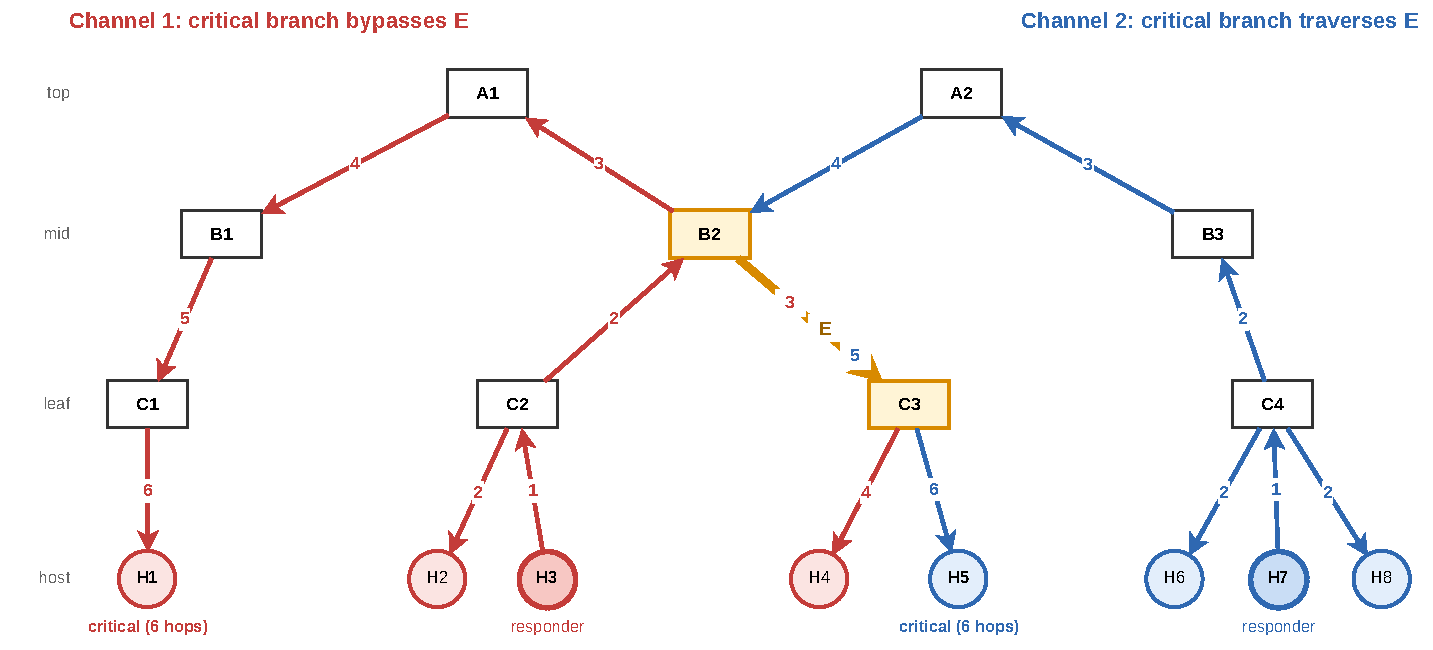
\includegraphics[width=0.94\linewidth]{img/eval/asym_2348.pdf}
\caption{\texttt{asym-2348}：用 responder 放置改变同一条队列在完成
反馈中是否可见。橙色为被测 egress $E$；配对放置保持成员、流量和 $E$
不变，仅 responder 位置使最慢分支绕过 $E$（红）或经过 $E$（蓝）。}
\label{fig:asym-2348}
\end{figure*}

\parab{过滤的公平性代价取决于控制律.}
最后，我们在同一 $E$ 上运行两个持续 backlogged 的四-rank channel。
两个 placement 采用共同的 $[1.92,5.76)$~ms 墙钟测量窗，并在 5.76~ms
同时停止发放新 offset 后排空所有已发 credit。主指标只计 completion
timestamp 落入该固定窗口的 logical bytes，不再使用各 job 自身的
submit-to-finish span，因而不包含先完成者独占的尾段。

\begin{table*}[t]
\centering
\caption{共享链路 $E$ 的反馈可见性对公平性与链路效率的影响。每个指标
的两列中，两条 channel 的流量均经过并竞争同一个 $E$：one-sided
feedback 表示只有 Channel~2 的 max-completion feedback 能感知 $E$ 上
的排队，two-sided feedback 表示双方的 feedback 都能感知。Channel~1
share 的 50\% 表示均分；aggregate completed goodput 把相同固定窗口内
两条 channel 完成的 logical bytes 相加后除以窗口长度，不再归一化。
DCQCN-style 使用 20 个 paired RNG run，其 Channel~1 share 唯一非零的
Student-t 95\% CI 为 0.003 percentage points；其余控制器的事件序列
确定，各运行一次。}
\label{tab:cc-asym}
\small
\pgfplotstabletypeset[
  col sep=comma,
  columns={controllerLabel,hiddenShare,visibleShare,
    hiddenAggregateGbps,visibleAggregateGbps},
  columns/controllerLabel/.style={
    string type,column name={Controller},column type=l,
  },
  columns/hiddenShare/.style={
    column name={One-sided feedback},
    fixed,fixed zerofill,precision=2,column type=r,
  },
  columns/visibleShare/.style={
    column name={Two-sided feedback},
    fixed,fixed zerofill,precision=2,column type=r,
  },
  columns/hiddenAggregateGbps/.style={
    column name={One-sided feedback},
    fixed,fixed zerofill,precision=1,column type=r,
  },
  columns/visibleAggregateGbps/.style={
    column name={Two-sided feedback},
    fixed,fixed zerofill,precision=1,column type=r,
  },
  every head row/.style={
    before row={
      \toprule
      & \multicolumn{2}{c}{Channel~1 share of completed goodput (\%)}
      & \multicolumn{2}{c}{Aggregate completed goodput (Gbps)}\\
      \cmidrule(lr){2-3}\cmidrule(lr){4-5}
    },
    after row=\midrule,
  },
  every last row/.style={after row=\bottomrule},
]{plots/data/pgf/cc.csv}

\end{table*}

\Cref{tab:cc-asym} 中，one-sided feedback 下 Swift 获得 93.0\% 的
completed goodput；改为 two-sided feedback 后，其 share 回到 50.0\%，
两种放置下的 aggregate completed goodput 分别为 199.0 和
198.6~Gbps——强烈的份额偏置来自瓶颈容量的重新分配，而非共享链路
空闲。Oscar 和 TIMELY 的 share 变化分别为 4.81 和 3.91 percentage
points，低于预注册的 5-point``明显偏置''门槛，我们不把它们写成强公平
性失效；其中只有 TIMELY 的 aggregate completed goodput 同时从 182.3
提高到 198.6~Gbps。DCQCN-style 的两个 placement 分别为
$49.975\pm0.003$\% 和 50.000\%，近似不受放置影响。全部 46 次运行均无
PFC 或协议错误。因此，branch-slack filtering 是信号本身的确定性边界，
但它是否放大为可见的带宽偏置取决于控制律；在该构型中，只有 Swift 达到
预注册的强边界阈值。

\section{可靠性}
\label{ssec:eval-reliability}

\parab{物理 communicator 生命周期.}
固定-$N=4$ 实验在五个新进程中交替创建和销毁 group~0/1，每个进程运行
25 轮，共验证 500 个 communicator 和 2,000 个 rank lifecycle。rank-churn
实验保持四个物理 rank、两个 poller、EAL 进程、NIC 队列和 FPGA 镜像不变，
在 group~0/3 上交替 $N=4$ 与 $N=2$，再次验证 500 个 communicator 和
2,000 个 rank lifecycle。两组实验均无残留 completion state、结构错误、
Tofino/DCMAC 错误、accelerator configuration write 或 image reload。
该结果验证 endpoint-only 建组、销毁和 message epoch 复用，不作吞吐或
建组时延声明。

\parab{物理故障证据边界.}
归档的三-rank DPDK fault-proxy 实验对七种定向竞态各运行五次，35 个
attempt 全部得到 105/105 个 PASS rank，覆盖相应 endpoint state
machine；但该实验早于最终 endpoint 源码，其三-NIC proxy 布线也已被
V80 拓扑替换。当前单层与两层镜像在正式运行中都实际执行过一般
recovery，但没有重跑这七种精确注入；本文因此不把旧 proxy 结果当作当前
routed 实现的定向故障验收，完整故障矩阵由以下包级实验给出。

包级仿真部分在 U200 上固定 16 ranks、单 job、单树、256-MiB message、
Swift 和 65,536 slots，只注入丢包、straggler 或 requester crash。
normal credit 的 cutover deadline 和 repair trigger/END 的 RTO 均为
10~ms，timeout 敏感性实验单独改变前者。结果量化所测有限故障下的恢复
代价和正确性边界。

\parab{有限丢包均能完成，但 repair 很快成为主成本.}
我们在 host-facing 和 tree 链路的两个方向独立注入 per-hop Bernoulli
loss，每个非零点包含 20 个 RNG run；实际 drop denominator、packet
class 和有向链路计数在每次运行中闭合。安装 loss model 但令 $p=0$
时，goodput 为 180.9~Gbps。\Cref{fig:loss} 显示，$p=0.01\%$ 时两个
scope 分别达到 $62.7\pm5.3$ 和 $65.8\pm4.7$~Gbps；$p=1\%$ 时约
27.6\% 的 offset 由 repair 提交，goodput 降至 4.10~Gbps，逐跳 wire
bytes 相对 $p=0$ 增加约 60.5\%。5\% 压力点仍全部完成，但 repair 比例
达到 80.6--80.7\%，goodput 只剩 0.78--0.81~Gbps。

\begin{figure*}[t]
\centering
\resizebox{\linewidth}{!}{%
\begin{tikzpicture}
\begin{groupplot}[
  group style={group size=2 by 1,horizontal sep=1.25cm},
  arbor axis,arbor panel,
  width=8.0cm,height=4.7cm,
  xmode=log,
  xmin=0.006,xmax=7,
  xtick={0.01,0.1,1,5},xticklabels={0.01,0.1,1,5},
  xlabel={Per-hop packet loss (\%)},
]
\nextgroupplot[
  title={(a) Logical goodput},
  ylabel={Goodput (Gbps)},ymin=0,ymax=75,
  ytick={0,25,50,75},
  legend to name=g6losslegend,legend columns=2,
  legend style={/tikz/every even column/.append style={column sep=5pt}},
]
\addplot[ArborBlue,thick,mark=*,error bars/.cd,y dir=both,y explicit]
  table[col sep=comma,x=loss_pct,y=host_goodput_gbps,
    y error=host_goodput_ci95]
  {plots/data/pgf/reliability.csv};
\addlegendentry{Host-facing links}
\addplot[ArborOrange,thick,dashed,mark=square*,
  error bars/.cd,y dir=both,y explicit]
  table[col sep=comma,x=loss_pct,y=tree_goodput_gbps,
    y error=tree_goodput_ci95]
  {plots/data/pgf/reliability.csv};
\addlegendentry{Tree links}

\nextgroupplot[
  title={(b) Recovery work},
  ylabel={Offsets committed by repair (\%)},ymin=0,ymax=90,
  ytick={0,20,40,60,80},
]
\addplot[ArborBlue,thick,mark=*,error bars/.cd,y dir=both,y explicit]
  table[col sep=comma,x=loss_pct,y=host_repair_pct,
    y error=host_repair_ci95]
  {plots/data/pgf/reliability.csv};
\addplot[ArborOrange,thick,dashed,mark=square*,
  error bars/.cd,y dir=both,y explicit]
  table[col sep=comma,x=loss_pct,y=tree_repair_pct,
    y error=tree_repair_ci95]
  {plots/data/pgf/reliability.csv};
\end{groupplot}
\node[anchor=south,yshift=26pt] at (group c1r1.north east)
  {\ref{g6losslegend}};
\end{tikzpicture}%
}

\caption{Host-facing 或 tree 链路双向独立随机丢包下的 20-run 均值和
Student-t 95\% CI。概率是每条所选有向链路上 eligible Arbor packet 的
per-hop loss；5\% 为压力点。}
\label{fig:loss}
\end{figure*}

\parab{Cutover deadline 过短或过长都会增加完成时间.}
我们丢弃一份 master，并交叉扫描 $\{2,10\}\times p99$ clean RTT 和固定
50-ms deadline，以及 $\{0,0.5,2\}\times p99$ requester delay；repair
RTO 始终固定为 10~ms。$2\times p99$ 把 32,682--32,768 个 offset 提前
转入 repair，goodput 为 68.5--68.9~Gbps；$10\times p99$ 只触发
129--175 次 repair，达到 173.5--185.7~Gbps。50-ms deadline 只 repair
丢失的那一个 offset，但 CCT 被该 deadline 拉长到 50.1~ms。normal
cutover 和 repair 重传因此必须使用独立 timer。

\parab{定向竞态保持单次提交.}
仿真侧的 18 个 packet-level 用例覆盖六种原语，以及 master、
payload+credit、\texttt{REGISTER\_ACK}、\texttt{END}/\texttt{END\_ACK}
和 repair trigger 的丢失、重复或迟到。跨级 master 丢失产生一次
repair trigger 和一次 repair commit；Broadcast 和 AllGather 的 push
offset 已在首发时 self-commit，丢失接收副本只重放 payload，没有二次
commit。一条 tree branch 暂停 2~ms 时，112 个 offset 转入 repair，
运行仍以 72.5~Gbps 完成。把一个 requester 限制到线速的 50\% 和
10\% 时，整组 goodput 分别为 97.4 和 19.8~Gbps；永久 crash 在
100~ms 截止前不提交缺少输入的结果。272 个有限故障点全部完成，且没有
PFC、\texttt{AGG\_MISS}、live overwrite 或协议违例；crash 边界不计入
成功均值。

\section{局限性}

评估有五项边界。第一，ns-3 不执行 payload 数值运算；其结果验证协议、
状态和链路线量，不能替代物理 FPGA 的 FP32 正确性、吞吐或资源证据。
第二，该 ns-3 fork 把 PRE 副本逐份计入同一 ingress queue；PFC pause 是
仿真中的真实事件，其 headroom 不能直接解释为商用交换机所需的物理
buffer。第三，没有一种端侧拥塞控制算法及参数配置在所有 group size、
拓扑和并发度上同时最优；正文参数按实验族在独立 calibration 上冻结，并
统一用于该实验族的 evaluation seed。第四，物理原型只有一块 V80、四个
rank 和每端口 100-GbE 的线速上限；正式性能运行以物理锁和进程门排除
ns-3、Vivado/JTAG 及其它 endpoint workload，所得 routed timing、资源和
吞吐不能外推为生产集群结果。第五，ATP-8K 和 SwitchML-8K 是按论文数据面
语义构建的独立 FPGA/endpoint 实现，不是原作者代码；物理结果支持相同
testbed 上的实现比较，不证明对原系统所有功能和优化的复现。当前 routed
镜像尚未重跑七种精确故障注入；两层动态选路虽有物理消融，但硬件计数器只
支持 500-ms 时间分辨率，控制律替换与更细响应时间仍采用包级仿真证据。

\FloatBarrier
